\section{\label{sec:abstract}Abstract}

\noindent We present a joint multi-robot trajectory optimizer that can compute trajectories for tens of robots in aerial swarms within a small fraction of a second. The computational efficiency of our approach is built on breaking the per-iteration computation of the joint optimization into smaller, decoupled sub-problems and solving them in parallel through a custom batch optimizer. We show that each of the sub-problems can be reformulated to have a special Quadratic Programming structure, wherein the matrices are shared across all the problems and only the associated vector varies. As result, the batch solution update rule reduces to computing just large matrix vector products which can be trivially accelerated using GPUs. We validate our optimizer's performance in difficult benchmark scenarios and compare it against existing state-of-the-art approaches. We demonstrate remarkable improvements in computation time its scaling with respect to the number of robots. Moreover, we also perform better in trajectory quality as measured by smoothness and arc-length metrics.

{\small \textit{(Published in the journal Frontiers in Robotics and AI, Vol. 9, 2022.  \cite{self-gpu-mat}, also presented at the DMMAS workshop, International Conference on Intelligent Robots and Systems (IROS) 2022.)}}    
%\tableofcontents


\section{Introduction}

Deployment of multiple aerial vehicles such as quadrotors is critical for applications like search and rescue and exploration and mapping of large areas \citep{schranz2020swarm}. Over the last decade, robot fleets have also become ubiquitous in applications like ware-house automation that have a substantial economic impact on society \citep{bolu2021adaptive,priority_seq}. Furthermore, with the advent of connected autonomous cars, it becomes imperative also to view urban mobility as a multi-robot system \citep{zhou2017collision}. A fundamental component of any multi-robot system is the coordination planning that guides individual robots between their start and goal locations while avoiding collisions with the environment and other robots. In this chapter, we adopt the optimization perspective for multi-robot motion planning \citep{aks_ral21}. In this context, the existing approaches broadly fall into two spectra. On one end, we have the centralized approaches wherein the trajectory of all the robots are computed together. The centralized approach can be further subdivided into sequential \citep{incremental_scp_how}, \cite{park2020efficient} and joint optimization \citep{rafaella_scp}, \citep{aks_ral21} respectively depending on whether the trajectories of the robots are computed one at a time or simultaneously. On the other end of the spectrum, we have online distributed model predictive control (DMPC) \citep{dmpc_carlos}, \citep{dmpc_epfl} based approaches wherein each individual robot computes its trajectories in a decoupled manner based on the trajectory prediction of the other robots in the environment. In some works, the prediction module is replaced by robots communicating their current trajectory with each other \citep{dmpc_carlos_2}. 

Centralized approaches, especially the joint optimization variants, provide a rigorous treatment of the collision avoidance constraints and access a larger feasible space formed by all trajectory variables of all the robots. However, joint optimization quickly becomes intractable as the number of robots increases \citep{chen2015decoupled}. In contrast, the distributed MPC approaches can run in real-time but can lead to oscillatory behaviors, and consequently, low success rates of collision avoidance \citep{dmpc_carlos}, \citep{dmpc_carlos_2}. This is because the trajectories computed at each control cycle by any robot are only collision-free with respect to the predicted (or prior communicated ) trajectories of other robots and not the actual trajectories followed by them. 

Our main motivation in this chapter is to improve the computational tractability of multi-robot trajectory planning using a distributed optimization approach to the extent that it becomes possible to compute trajectories for tens of robots in densely cluttered environments in a few tens of milliseconds. To put in context, the said timing is several orders of magnitude faster than some of the existing approaches for joint multi-robot trajectory optimization \citep{rafaella_scp}, \citep{alonso_mora_nips_multi}. Such improvements in computation time would ensure the applicability of our approach for even online re-planning besides the standard use case of computing offline global trajectories for the robots. For example, consider a scenario wherein each robot uses local real-time planners such as Dynamic Window Approach \citep{dwa} or DMPC \citep{dmpc_carlos} to avoid collisions with other robots in a distributive manner. Our approach could provide global re-planning for the local planners at more 5Hz. or more.

On the application side, our main focus is on coordination of multiple quadrotors, typically for applications like search and rescue and coordinated exploration. These applications require point-to-point, collision-free navigation and forms the main benchmark in our experiments. However, our algorithm can be useful for coordination of multiple wheeled mobile robots and even autonomous cars.


% An improvement in joint multi-robot trajectory optimization will be 






% Furthermore, the trajectories computed from our approach can also be used to warm-start the distributed MPC approaches.



\noindent \textbf{Contributions:}
The computational efficiency of our approach is built on several layers of reformulation of the underlying numerical aspects of the joint multi-robot trajectory optimization. We summarize the key points and the benefits that it leads to below.
 
\noindent \textbf{Algorithmic:} Our main idea is to break the per-iteration computation of the joint multi-robot trajectory optimization into smaller, distributed sub-problems by leveraging the solution computed in the previous iterations. Although similar ideas have appeared in many existing works \citep{alonso_mora_nips_multi}, \citep{dmpc_carlos_2}, a core challenge remains: how to efficiently solve the decoupled problem arising at each iteration in parallel. The basic assumption is that the decoupled optimizations can be parallelized across separate CPU threads \citep{alonso_mora_nips_multi}. However, our recent works have shown that such a parallelization approach does not scale well with an increase in the number of problems \citep{aks_behavior_ral22}. The inherent limitation stems from the available CPU cores and thread synchronization issues. 

Thus our main algorithmic contribution in this chapter lies in deriving a novel optimizer that can be efficiently run in a batch setting. In other words, our optimizer can take a set of decoupled optimization problems and vectorize the underlying numerical computations across multiple problem instances. Consider an optimizer that solves a given problem by adding two vectors as a hypothetical example. We can trivially vectorize the computation over different problem instances by stacking each problem's vectors together in the form of a matrix and adding them together. Moreover, this matrix addition can be easily parallelized over GPUs for many problem instances. Our proposed optimizer achieves similar vectorization but for a set of difficult non-convex sub-problems, resulting in each iteration of joint multi-robot trajectory optimization. Specifically, we show that solving the decoupled sub-problems predominantly reduces to solving novel equality constrained quadratic programming (QP) problems under certain collision constraint reformulations. The novelty of the QPs stems from the fact that they all share the same matrices (e.g., Hessian), and only the vectors associated with the QPs vary across the sub-problems. We show that solving all the QP sub-problems in one shot reduces to computing one large matrix-vector product that can be trivially parallelized over GPUs using off-the-shelf linear algebra solvers.  


\noindent \textbf{Applied:} We release our entire implementation for review and to promote further research on this problem. We also release the benchmark data sets used in our simulations.

\noindent \textbf{State-of-the-art Performance} We compare our GPU accelerated optimizer with two strong baselines  \citep{park2020efficient,aks_ral21} and show massive improvement in computation time while being competitive in trajectory quality as measured by metrics like arc-length and smoothness. Our first comparison is with \citep{park2020efficient} that uses a sequential approach for multi-robot trajectory optimization. Our computation time is at least $76.48\%$ lower than that of \citep{park2020efficient} for a smaller problem size involving $16$ robots. Moreover, the performance gap increases substantially in our favor as we increase the number of robots and make the environment more cluttered by introducing more static obstacles. We observe similar trends in trajectory arc-length and smoothness comparison between the two approaches. Our second comparison is with \citep{aks_ral21} that searches directly in the feasible joint space formed by all the pair-wise collision avoidance constraints. Our proposed optimizer shows improved scalability over \citep{aks_ral21} for a larger number of robots while being also superior in trajectory arc length and smoothness.

\section{Problem Formulation and Related Work}
This section introduces the general problem formulation for multi-robot trajectory optimization. We subsequently use the problem set-up to review existing works and contrast our optimizer with them. We begin by summarizing the main symbols and notations used throughout the chapter.

\subsection{Symbols and Notations}
\noindent In this chapter, the lower normal and bold letters denote the scalars and vectors, respectively, while the upper bold case variants represent matrices. The left and right super-scripts denoted by $k$ and $T$ will be used to denote the iteration index of the optimizer and transpose of the vectors and matrices. The time-stamp of any variable will be denoted by $t$. The symbol $\left\Vert \textbf{.} \right\Vert_{2}$ stands for $l_{2}$ norm. We summarize some of the main symbols in Table \eqref{table_1} while some are also introduced in their first place of use. At some places, we perform a special construction where time-stamped variables are stacked to form a vector. For example, $\textbf{x}_i$ will be formed by stacking $x_i(t)$ at different time instants.


\subsection{Robot Kinematics}
\noindent Our optimizer is designed for robots with holonomic motion models. That is, the motion along each axis is decoupled from each other. This is a common assumption made in quadrotor motion planning. Many commercially available wheeled mobile robots also have similar kinematic model. Under certain conditions, even motion planning for car-like vehicles also adopt similar kinematic model and thus our optimizer is suitable for those as well \cite{frenet_planner}.


\subsection{Trajectory Optimization }
\noindent For holonomic robots modeled as series of integrators, the joint trajectory optimization can be formulated in the following manner.

\begin{subequations}
\begin{align}
\min_{x_{i}(t), y_{i}(t), z_{i}(t)} \sum_{t, i} \Big(\ddot{x}_{i}^2(t)+\ddot{y}_{i}^2(t)+\ddot{z}_{i}^2(t)\Big),\label{cost_multirobot} \\
\Big(x_i(t_0), \dot{x}_i(t_0), \ddot{x}_i(t_0), y_i(t_0), \dot{y}_i(t_0), \ddot{y}_i(t_0), z_i(t_0), \dot{z}_i(t_0), \ddot{z}_i(t_0)) = \textbf{b}_{o, i}, \forall i \label{initial_boundary_cond} \\
\Big(x_i(t_f), \dot{x}_i(t_f), \ddot{x}_i(t_f), y_i(t_f), \dot{y}_i(t_f), \ddot{y}_i(t_f), z_i(t_f), \dot{z}_i(t_f), \ddot{z}_i(t_f)) = \textbf{b}_{f, i}, \forall i \label{final_boundary_cond} \\
  -\left(\begin{matrix}
 x_i(t)-x_j(t)\\
 y_i(t)-y_j(t)\\
 z_i(t)-z_j(t)\\
 \end{matrix}\right)^T\textbf{S}\left(\begin{matrix}
 x_i(t)-x_j(t)\\
 y_i(t)-y_j(t)\\
 z_i(t)-z_j(t)\\
 \end{matrix}\right)+1 \leq 0, \forall t,  \{i,j \in \{1,2,...,n_{r}\}, j \neq  i\} \label{coll_multirobot}, \textbf{S} = \begin{bmatrix}
 a^2 & 0 & 0 \\
 0 & a^2 & 0 \\
 0 & 0 & b^2 \\
 \end{bmatrix}
 \end{align}
\end{subequations}

\noindent The cost function (\ref{cost_multirobot}) minimizes the squared norm of the acceleration at each time instant for all the robots. The equality constraints  \eqref{initial_boundary_cond}-\eqref{final_boundary_cond} enforces the initial and final boundary conditions on positions, velocity, and accelerations on each robot trajectory. The pair-wise collision avoidance constraints are modeled by inequalities (\ref{coll_multirobot}), wherein we have assumed that the robots are shaped as axis-aligned spheroids with axis dimensions $(a, a, b)$. For the ease of exposition, we consider all robots to have the same shape. Extension to a more general setting is trivial. The constraints  (\ref{coll_multirobot})  are typically enforced at pre-selected discrete time-stamps, and thus a fine resolution of discretization is necessary for accurately satisfying the constraints. For now, we do not consider any static obstacles in the environment in the formulation above. The extension is trivial as static obstacles can be considered robots with zero velocity and whose trajectories are not updated within the optimizer's iteration.

Let the trajectory of each robot along each motion axis $x, y, z$ be parameterized through $n_v$ number of variables. For example, these variables could be time-stamped way-points representing the trajectory or the coefficients of their polynomial representation (see \eqref{param}). Then, for a set-up with $n_r$ number of robots and a planning horizon of $n_p$, optimization (\ref{cost_multirobot})-(\ref{coll_multirobot}) involves $n_r*n_v$ variables, and $18*n_r$ equality constraints. The number of pair-wise collision constraints would be ${n_r\choose{2}}*n_p$. 

The number of decision variables in optimization (\ref{cost_multirobot})-(\ref{coll_multirobot}) scales linearly with the number of robots. Although this increase poses a computational challenge, the main difficulty in solving the optimization stems from the non-convex pair-wise collision avoidance constraints (\ref{coll_multirobot}) as the rest of the cost and constraint functions are convex. Moreover, the number of collision avoidance constraints increases exponentially with the number of robots. Existing works  \citep{rafaella_scp,aks_ral21, incremental_scp_how, priority_seq, park2020efficient} have adopted different simplifications on the collision avoidance constraints to make multi-robot trajectory optimization more tractable. We thus next present a categorization of these works based on the exact methodology used.

\subsection{Literature Review}
\subsubsection{Joint Optimization with Conservative Convex Approximation}
\noindent The most conceptually simple approach is to solve (\ref{cost_multirobot})-(\ref{coll_multirobot}) as one large optimization problem, wherein the trajectory of every robot is computed in one shot. Authors in \citep{rafaella_scp} simplified the joint optimization by deriving a conservative affine approximation of the collision avoidance constraints (\ref{coll_multirobot}) and consequently reducing  (\ref{cost_multirobot})-(\ref{coll_multirobot}) to a sequence of QPs. As a result, their solution process becomes somewhat tractable for a moderate number of robots ($\approx 10$). However, the computation time of \citep{rafaella_scp} scales poorly because the number of affine constraints still increases exponentially with the number of robots. Our prior work \citep{aks_ral21} substantially improved the scalability of joint multi-robot trajectory optimization by reformulating the Euclidean collision constraints (\ref{coll_multirobot}) into polar form and augmenting them into the cost function by using concepts from the Alternating Direction Method of Multipliers (ADMM). Moreover, we showed that such reduction allowed one-time offline caching of the most expensive parts of the computation. As a result, \citep{aks_ral21} achieved over two orders of magnitude speed-up over \citep{rafaella_scp} for 16 robots. The current proposed work provides a further significant improvement over \citep{aks_ral21} in computation time and trajectory quality.

\subsubsection{Sequential Optimization}

Sequential planners plan for only one robot at a time. At any given planning cycle, the previously computed robot trajectories are considered dynamic obstacles for the currently planned robot. As a result, these approaches ensure that the number of decision variables does not increase with robots. Moreover, the number of collision avoidance constraints increases linearly as the planning cycle progresses. However, note that the linear increase in the number of constraints does not translate to similar scaling in computation time. Even state-of-the-art interior-point solvers have cubic complexity with respect to the number of constraints.

A critical disadvantage of sequential planners is that each subsequent robot has access to less feasible space to maneuver. As a result, optimization problems become progressively constrained as the planning cycle progresses, leading to potential infeasibility. Authors in \citep{incremental_scp_how} tackle this problem by developing an incremental constraint tightening approach. The authors integrate a subset of collision avoidance constraints into the optimization problem, and the size of this set is gradually increased based on the actual collision residuals.

Sequential planners naturally have the notion of priority, and these can be chosen carefully for improved performance. For example, \citep{priority_seq} adopts a priority-based optimization method in which the robots are divided into groups/batches with pre-determined priorities, and the trajectory optimization problem is solved from the highest to the lowest priority group. Similar approach was adopted in \citep{park2020efficient}. Performing sequential planning over a small batch of robots reduces its conservativeness. On the other hand, it introduces an additional challenge of ensuring collision amongst the robots in a given batch. Authors in \citep{park2020efficient} tackle this bottleneck by leveraging graph-based Multi-robot Path Finding (MAPF) methods.



% and solves the collision avoidance problem with respect to all other dummy robots in each iteration. In the next iteration, the robots in the current batch are used as dummy robots, and the process is sequentially repeated. The collision avoidance constraints are expressed in terms of Bernstein polynomials and the initial trajectory is planned using a graph-based Multi-robot Path Finding (MAPF) method. We benchmark our approach against this algorithm and achieve remarkable improvements in computation time by leveraging GPU computations, while maintaining comparable trajectory quality.


% Priorities are assigned based on the occurrence of robot triplets whose trajectories are coupled due to their closeness to one another.
\subsubsection{Distributed Optimization} 

Distributed optimizers at each iteration, break (\ref{cost_multirobot})-(\ref{coll_multirobot}) into decoupled smaller problems. For example, see \citep{alonso_mora_nips_multi}, \citep{multi_robot_1}. The key insight upon which all existing works build is that the only coupling between different robots stem from the pair-wise collision constraints (\ref{coll_multirobot}) \citep{multi_robot_1}. Thus, we if we discard this coupling, (\ref{cost_multirobot})-(\ref{coll_multirobot}) can be easily reduced to $n_r$ number of decoupled optimizations. One way to achieve the said decoupling is to let each robot make prediction of how the trajectories of other robots are going to look in the immediate next iterations and use that to simplify the collision avoidance constraints. More formally, let $(\overline{x}_j(t), \overline{y}_j(t), \overline{z}_j(t) )$ be the predicted position of $j^{th}$ robot at time $t$. Then, the collision avoidance constraints can be simplified as (\ref{distributed_coll}). 


\begin{figure}
    \centering
    {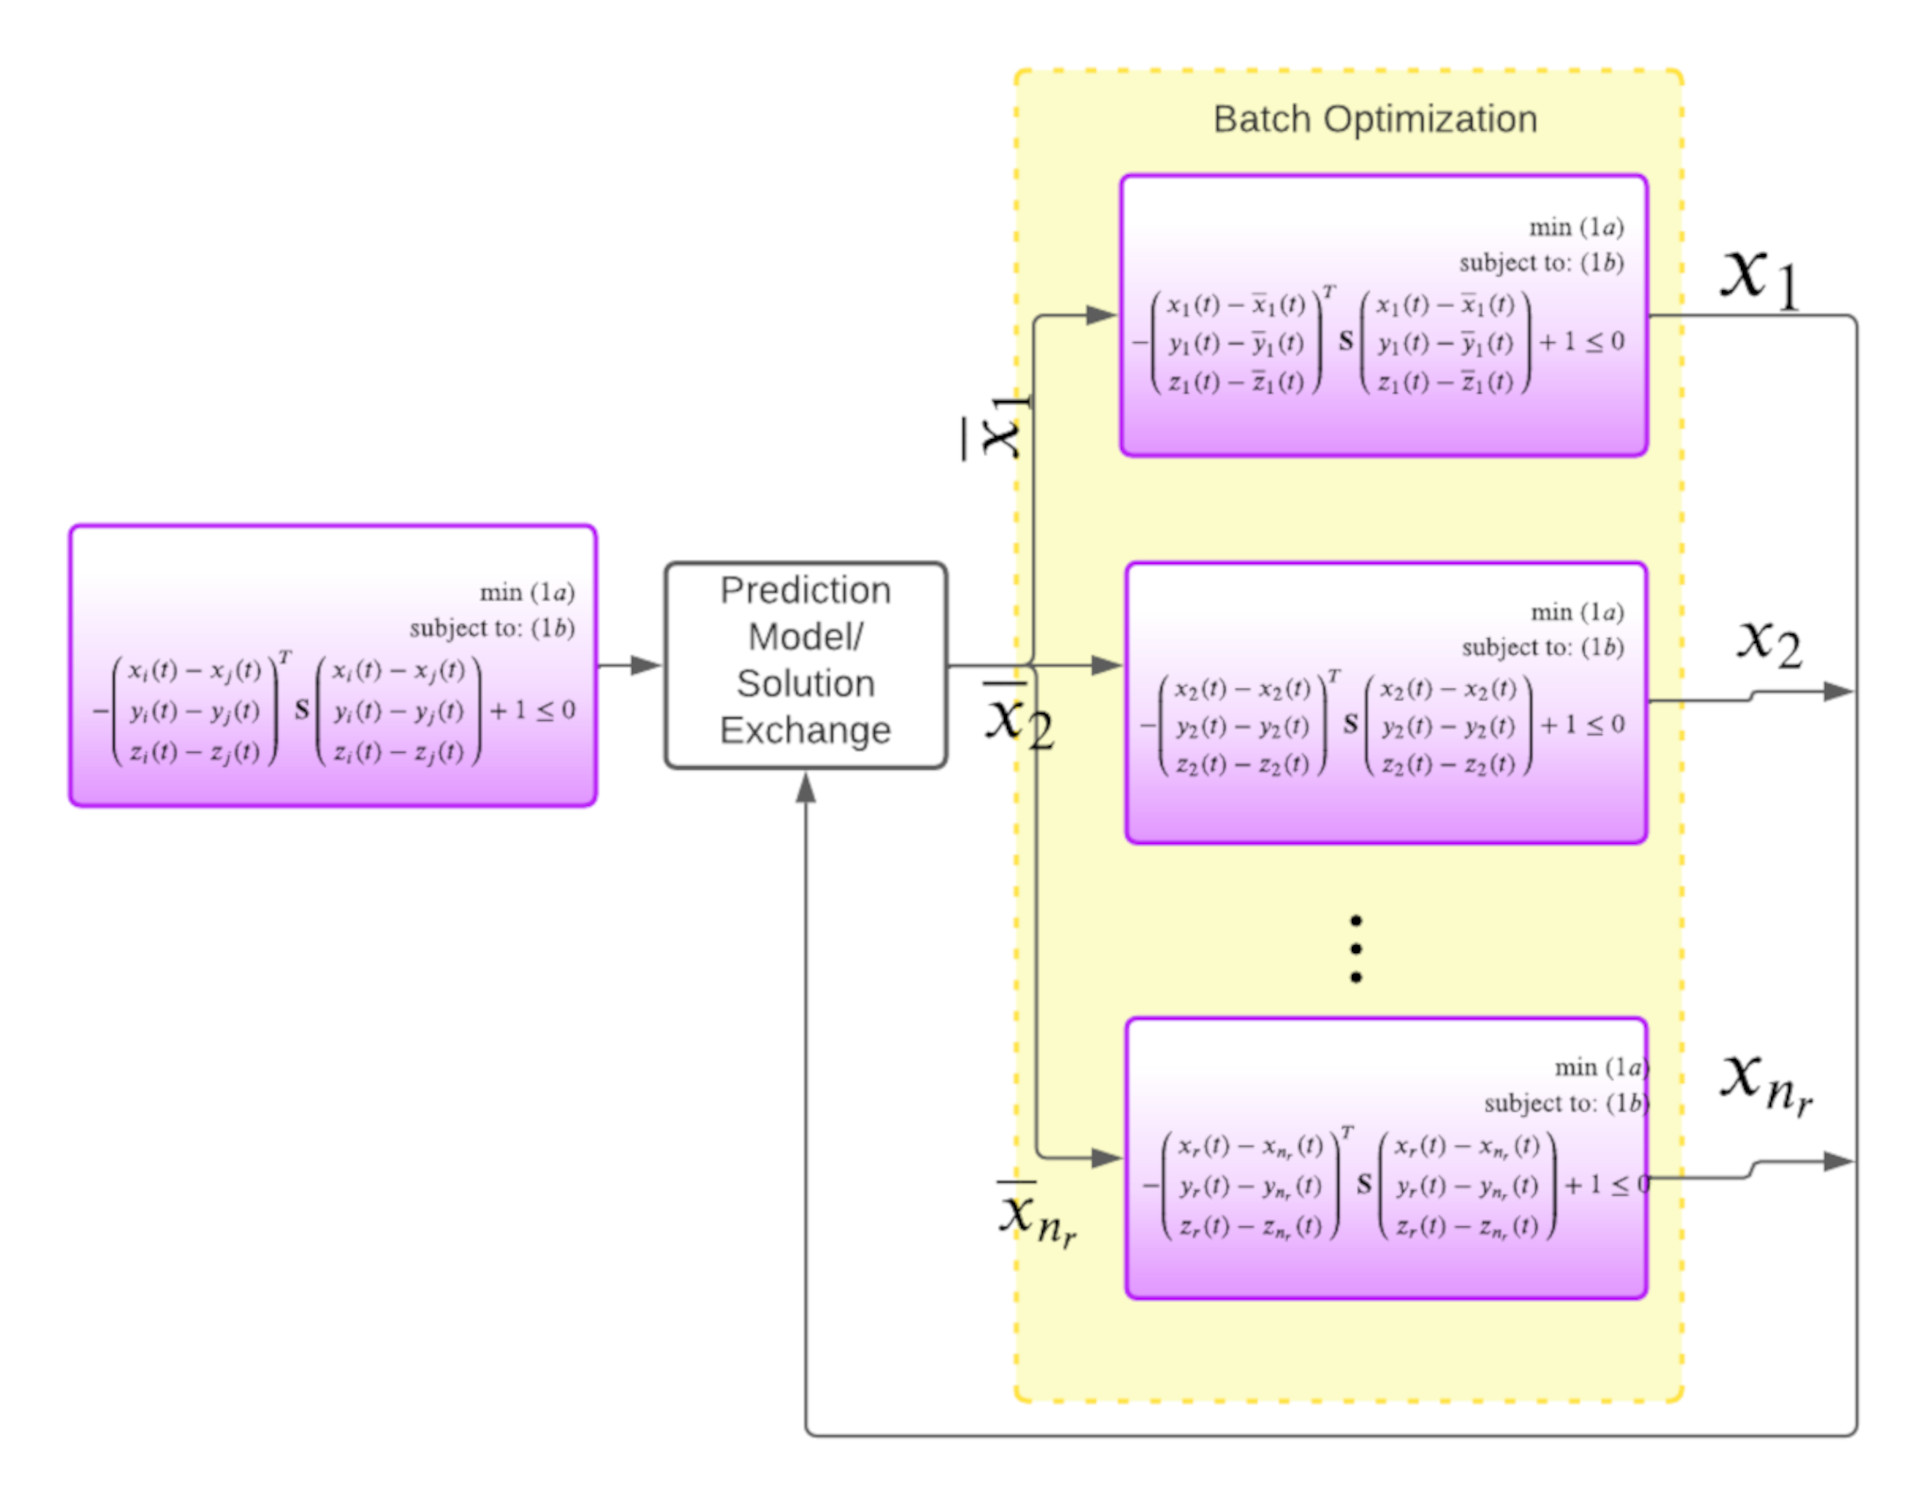
\includegraphics{figures/gpu_mat/pipeline.jpg}} 
    \caption[GPU multi-robot optimizer pipeline]{ Figure shows our approach for breaking the joint optimization (first block) at each iteration into decoupled sub-problems (third group of blocks). Each robot exchanges their current computed trajectories with each other. For the next iteration, robots will use the communicated trajectories to frame their collision avoidance constraints. Thus, in this manner, we can avoid the inter-robot coupling in collision constraints. Our core novelty in this chapter is a batch optimizer that can solve all the decoupled problems in parallel over GPUs. It is also possible to replace the trajectory exchange set-up with a model that predicts the nature of the robot trajectories in the immediate next iteration. Note that we only show the $x$ component of the trajectory purely to maintain clarity in the figure.}
    \label{fig: figure_block_diagram}
\end{figure}

\begin{align}
    \left(\begin{matrix}
    x_i(t)-\overline{x}_j(t)\\
 y_i(t)-\overline{y}_j(t)\\
 z_i(t)-\overline{z}_j(t)\\
 \end{matrix}\right)^T\textbf{S}\left(\begin{matrix}
 x_i(t)-\overline{x}_j(t)\\
 y_i(t)-\overline{y}_j(t)\\
 z_i(t)-\overline{z}_j(t)\\
 \end{matrix}\right)+1 \leq 0
 \label{distributed_coll}
\end{align}

\noindent Note that $(\overline{x}_j(t), \overline{y}_j(t), \overline{z}_j(t) )$ is a known constant in (\ref{distributed_coll}). Fig.\ref{fig: figure_block_diagram} shows how the process of using (\ref{distributed_coll}) to formulate decoupled optimization problems for each robot. Existing works differ in their method of computing the prediction $(\overline{x}_j(t), \overline{y}_j(t), \overline{z}_j(t) )$. The simplest possibility is to set it as the solution obtained in the previous iteration \citep{alonso_mora_nips_multi}, which is what we use in our formulation as well.

\subsubsection{Online DMPC} 
\noindent DMPC approaches are the online variants of the distributed optimization approach. In other words, if we run one iteration of distributed optimization and let each robot move with the computed trajectory, we recover the DMPC works such as \citep{dmpc_carlos}, \cite{dmpc_carlos_2}. This insight also points to the main issue of DMPC. At each control cycle, imagine a robot $i$ receiving information (directly through communications or indirectly through prediction) about the trajectory that the other robot $j$ computed. Then it uses this information to construct collision avoidance constraints in its trajectory optimization set-up. However, robot $j$ will follow the same process and update its trajectory as well. Thus, essentially both robot $i$ and $j$ compute their motion based on outdated information about each other's behavior.

\subsubsection{Batch optimization over CPU Vs GPU}

Parallelization of a batch of optimization problems across CPUs and GPUs operates fundamentally differently, and both classes of approaches have been tried in existing works to speed up multi-robot trajectory optimization. Each CPU core is efficient at handling arbitrary numerical computations, and thus solving a batch of optimizations problems in parallel is conceptually simple. We can solve each problem in a separate thread without needing to make any change in the underlying numerical algebra of the optimizer \citep{aks_behavior_ral22}, \citep{alonso_mora_nips_multi}. As mentioned earlier, the scalability of CPU parallelization is limited by the number of cores (typical 6 in a standard laptop). On the other hand, GPUs have many cores, but these are primarily efficient at parallelizing primitive operations such as matrix-vector and matrix-matrix multiplication.
Moreover, GPUs excel in performing the same primitive operations over many data points. Thus, to fully leverage the compute power of GPUs, it is necessary to modify the underlying numerical aspect of an optimizer to fit the strengths of GPUs. For example, GPU acceleration of Newton's method requires adopting indirect matrix factorization over the more common direct approaches \citep{newton_gpu}. One optimization technique that trivially accelerates over GPUs is Gradient Descent (GD) since it boils down to just matrix-vector multiplication. Authors in \citep{rafaella_gpu} leverage this insight for developing a fast multi-robot trajectory optimization algorithm. One critical issue of \citep{rafaella_gpu} is that the proposed GD is very sensitive to hyper-parameters like weights of the different cost function, learning rate, etc.


    %\caption{Empirical validation of convergence of our optimizer. The figure shows the residual of $\Vert \textbf{F}\boldsymbol{\xi}_{1, i}-\textbf{g}_i\Vert$ averaged over all $i$ (agent index) and across different benchmarks.}

GPUs are designed using threads grouped into blocks, which are themselves organized as grids to parallelize computations for computational efficiency \citep{li_GPUmatmul}. The GPU first tiles an $n \times n$ matrix using $p \times q$ tiles indexed with a 2-dimensional index to multiply large matrices. The output of each tile in the result matrix is independent of other tiles, which allows for parallelization. The parallelized CUDA code uses a block of threads to compute each tile of the result matrix, and to compute the entire result matrix; it uses a $\frac{n}{p} \times \frac{n}{q}$ grid of thread blocks. Many threads and blocks in modern GPUs allow for simultaneous computation of tile outputs, allowing for a many-fold boost in the computation time required for large matrix multiplications. Most off-the-shelf GPU-based libraries have this inbuilt CUDA programming for parallel GPU computations and can be utilized for achieving computational speed-ups in matrix multiplications.


% Our approach in this chapter for solving the batch of distributed sub-problems arising at each iteration of multi-robot trajectory optimization is more sophisticated than a typical GD based optimizer. As, we


% We reduce the operations of batch optimization to solving a set of linear equations (see \eqref{over_2}).\color{black}


\section{Methods}
\subsection{Overview} \label{batch_QP_setup}
\noindent Similar to \citep{alonso_mora_nips_multi}, we break the joint multi-robot trajectory optimization (\ref{cost_multirobot})-(\ref{coll_multirobot}) into decoupled smaller sub-problems at each iteration. This is illustrated in Fig.\ref{fig: figure_block_diagram}. At a conceptual level, this decoupling process can be interpreted in the following manner: the robots communicate among themselves the trajectories they obtained in the previous iteration of the optimizer. Each robot then uses them to independently formulate their collision avoidance constraints. Our work differs from existing works in the way the decoupled problems illustrated in Fig.\ref{fig: figure_block_diagram} is solved. As mentioned before, a trivial approach to solving the sub-problems in parallel CPU threads is not scalable for tens of robots. In contrast, our main idea in this chapter is to develop a GPU accelerated optimizer that can solve a batch of optimization problems in one shot. 

In this sub-section, we aim to provide a succinct mathematical abstraction of our main idea. We discuss a special class of problems that are simple to solve in batch fashion. To this end, consider the following batch of equality constrained QPs, $ i\in \{1,2,...,n_r\}$.

\begin{align}
\min_{\boldsymbol{\xi}_{i}} \Big(\frac{1}{2}\boldsymbol{\xi}^{T}_{i}\overline{\textbf{Q}}\boldsymbol{\xi}_{i} + \overline{\textbf{q}}^{T}_{i}\boldsymbol{\xi}_{i}\Big), \qquad
 \text{st: } \overline{\textbf{A}} \boldsymbol{\xi}_{i} = \overline{\textbf{b}}_{i} \label{over_1}
\end{align}

\noindent In total, there are $n_r$ QPs to be solved, each defined over variable $\boldsymbol{\xi}_i$. The QPs defined in (\ref{over_1}) have a unique structure. The Hessian $\overline{\textbf{Q}}$ and the constrained matrix $\overline{\textbf{A}}$ are shared across the problems and only the vectors $\overline{\textbf{q}}_i$ and $\overline{\textbf{b}}_i$ varies across the batch. This special structure leads to efficient batch solution formulae. To see how, note that each QP in the batch can be reduced to solving the following set of linear equations.

\begin{align}
    \begin{bmatrix}
        \overline{\textbf{Q}} & \overline{\textbf{A}}^{T} \\ 
        \overline{\textbf{A}} & \textbf{0}
    \end{bmatrix} \begin{bmatrix}
        \boldsymbol{\xi}_{i}\\ \boldsymbol{\mu}_{i}
    \end{bmatrix} = \begin{bmatrix}
        \overline{\textbf{q}}_{i} \\ \overline{\textbf{b}}_{i}
    \end{bmatrix}, \qquad \forall i \in \{ 1,2,...,n_{r} \} \label{over_2}
\end{align}

\noindent where $\boldsymbol{\mu}_i$ are the dual optimization variables. Now, it can be observed that the matrix on the left-hand side of (\ref{over_2}) is independent of the batch index $i$, and thus, the solutions for the entire batch can be computed in one shot through \eqref{over_3}.

\begin{align}
\begin{bmatrix} 
\begin{array}{@{}c|c|cc@{}}
\boldsymbol{\xi}_{1} &...& \boldsymbol{\xi}_{n_{r}} \\ \boldsymbol{\mu}_{1} &...& \boldsymbol{\mu}_{n_{r}}
\end{array}
\end{bmatrix} =
    \overbrace{\left (\begin{bmatrix}
        \overline{\textbf{Q}} & \overline{\textbf{A}}^{T} \\ 
        \overline{\textbf{A}} & \textbf{0}
    \end{bmatrix}^{-1}\right )}^{matrix}
\overbrace{\begin{bmatrix}
\begin{array}{@{}c|c|cc@{}}
    \overline{\textbf{q}}_{1} & \overline{\textbf{q}}_{2}& ... & \overline{\textbf{q}}_{n_{r}}  \\
    \overline{\textbf{b}}_1 & \overline{\textbf{b}}_2 & ... & \overline{\textbf{b}}_{n_{r}} 
    \end{array}\end{bmatrix}}^{\text{stacked vectors}},
    \label{over_3}
\end{align}

\noindent where $|$ represents that the columns are stacked horizontally. The batch solution (\ref{over_3}) amounts to multiplying one single matrix with a batch of vectors. Furthermore, the matrix is constant, and its dimension is independent of the number of problems in the batch. Thus, operation (\ref{over_3}) can be trivially parallelized over GPUs using off-the-shelf libraries like JAX \citep{bradbury2020jax}.

\noindent \textbf{How it all fits:} In the next few sub-sections, we will show how the distributed sub-problems of (\ref{cost_multirobot})-(\ref{coll_multirobot}), shown in Fig.\ref{figure1} can be solved efficiently in a batch setting. Specifically, we reformulate these problems in such a way that the most intensive part of their solution process reduces to solving a batch of QPs with the special structure presented in (\ref{over_1}). 

\subsection{Collision Avoidance in Polar Form}
\noindent An important building block of our approach is rephrasing the collision avoidance constraints into the following polar representation from \citep{aks_ral21}, \citep{rastgar2020novel}.

\begin{align}
\textbf{f}_{c}(x_{i}(t),y_{i}(t)) = 
\left \{ \begin{array}{lcr}
x_{i}(t) - \overline{x}_{j}(t) - ad_{ij}(t)\sin{\beta_{ij}(t)}\cos{\alpha_{ij}(t)} \\
y_{i}(t) - \overline{y}_{j}(t) - ad_{ij}(t)\sin{\beta_{ij}(t)}\sin{\alpha_{ij}(t)} \\
z_{i}(t) - \overline{z}_{j}(t) - bd_{ij}(t)\cos{\beta_{ij}(t)}
\end{array} \right \},  \qquad  d_{ij}(t) \geq 1,
\label{fc} 
\end{align}

\noindent where $\alpha_{ij}(t), \beta_{ij}(t), d_{ij}(t)$  are unknown variables that will be computed by the optimizer along with each robot's trajectory. Physically, $\alpha_{ij}(t)$ and $\beta{ij}(t)$ represent the 3D solid angle of the line-of-sight connecting robot $i$ and $j$ based on the predicted motion of the latter. The variable $d_{ij}(t)$ is the ratio of the length of the line-of-sight vector with minimum safe distance $\sqrt{a^2+a^2+b^2}$ (see \citep{aks_ral21}).

\subsection{Proposed Reformulated Distributed Problem}
\noindent Using (\ref{fc}), we can reformulate the distributed sub-problems presented in Fig.\ref{figure1} for the $i^{th}$ robot in the following manner. We reiterate that $(\overline{x}_j(t), \overline{y}_j(t), \overline{z}_j(t)), \forall j\neq i $ is known based on the prediction of the trajectories of other robots.

\begin{subequations}
\begin{align}
\min_{ \scalebox{0.8}{$ x_{i}(t), y_{i}(t), z_{i}(t), d_{ij}(t),
\alpha_{ij}(t), \beta_{ij}(t)  $}}
\sum_t \Big(\ddot{x}^2_{i}(t)+\ddot{y}^2_{i}(t) + \ddot{z}^2_{i}(t) \Big), \label{acc_cost_reform}\\
 %\Tilde{\psi}(t)=\psi(t) \label{reformulate_psi}\\
\Big(x_i(t_0), \dot{x}_i(t_0), \ddot{x}_i(t_0), y_i(t_0), \dot{y}_i(t_0), \ddot{y}_i(t_0), z_i(t_0), \dot{z}_i(t_0), \ddot{z}_i(t_0)) = \textbf{b}_{o, i}, \forall i \label{initial_boundary_cond_reform} \\
\Big(x_i(t_f), \dot{x}_i(t_f), \ddot{x}_i(t_f), y_i(t_f), \dot{y}_i(t_f), \ddot{y}_i(t_f), z_i(t_f), \dot{z}_i(t_f), \ddot{z}_i(t_f)) = \textbf{b}_{f, i}, \forall i \label{final_boundary_cond_reform} \\
\textbf{f}_{c} \hspace{-0.1cm}: \hspace{-0.1cm}\left \{ \begin{array}{lcr}
x_{i}(t)-\overline{x}_{j}(t) -ad_{ij}(t)\sin{\beta_{ij}(t)}\cos{\alpha_{ij}}(t)\\
y_{i}(t)-\overline{y}_{j}(t) 
-ad_{ij}(t)\sin{\beta_{ij}(t)}\sin{\alpha_{ij}(t)} \\
z_{i}(t)-\overline{z}_{j}(t) -bd_{ij}(t)\cos{\beta_{ij}(t)}
\end{array} \right \} \label{coll_con} \\% \right \}
 d_{ij}(t) \geq 1, \qquad \forall t, j, \{j| j\in \{1,2,...,n_{r}\}, j \neq  i\} \label{collision_reform}
\end{align}
\end{subequations}

\subsubsection{Finite Dimensional Representation}
\noindent Optimization (\ref{acc_cost_reform})-(\ref{collision_reform}) is expressed in terms of functions and thus has the so called infinite dimensional representaton. To obtain a finite-dimensional form, we assume some parametric form for this functions. For
different $d_{ij}(t), \alpha_{a_{ij}}(t), \beta_{ij}(t) $, we assume a way-point paramterization. That is, these functions are represented through values at discrete time instants. The trajectories along each motion axis are represented as following polynomials.

\begin{equation}
\begin{bmatrix}
x_{i}(t_1)\\
x_{i}(t_2)\\
\vdots\\
x_{i}(t_{n_{p}})
\end{bmatrix} =\textbf{P} \textbf{c}_{x,i}, \qquad
\begin{bmatrix}
\dot{x}_{i}(t_1)\\
\dot{x}_{i}(t_2)\\
\vdots\\
\dot{x}_{i}(t_{n_{p}})
\end{bmatrix} = \dot{\textbf{P}}\textbf{c}_{x,i}, \qquad
\begin{bmatrix}
\ddot{x}_{i}(t_1)\\
\ddot{x}_{i}(t_2)\\
\vdots\\
\ddot{x}_{i}(t_{n_{p}})
\end{bmatrix} = \ddot{\textbf{P}}\textbf{c}_{x,i}.
\label{param}
\end{equation}

\noindent Similar expressions as (\ref{param}) can be written for the $y, z$ component of the trajectory as well. The matrix $\textbf{P}$ is formed with time dependent polynomial basis functions. Using (\ref{param}), we can re-write (\ref{acc_cost_reform})-(\ref{collision_reform}) in the following matrix form. 

\begin{subequations}
\begin{align}
 \min_{\boldsymbol{\xi}_{1,i}, \boldsymbol{\xi}_{2,i}, \boldsymbol{\xi}_{3,i}, \boldsymbol{\xi}_{4,i}} \Big(\frac{1}{2}\boldsymbol{\xi}_{1,i}^T\textbf{Q}\boldsymbol{\xi}_{1,i} \Big)\label{cost_matrix_form},  \\
  \textbf{A}_{eq}\boldsymbol{\xi}_{1,i} = \textbf{b}_{eq},   \label{eq_matrix_form}\\
  \textbf{F}\boldsymbol{\xi}_{1,i} = \textbf{g}_{i}(\boldsymbol{\xi}_{2,i},\boldsymbol{\xi}_{3,i}, \boldsymbol{\xi}_{4,i} ) \label{non_convex_equality_matrix-form},\\
 \boldsymbol{\xi}_{4,i}\geq \textbf{1}, \label{d_bound_matrix_form}
\end{align}
\end{subequations}

\noindent where, $\boldsymbol{\xi}_{1,i} = (\textbf{c}_{x,i}, \textbf{c}_{y,i}, \textbf{c}_{z,i}) $, $\boldsymbol{\xi}_{2,i} = \boldsymbol{\alpha}_{ij}$,  $\boldsymbol{\xi}_{3,i} = \boldsymbol{\beta}_{ij}$ and $\boldsymbol{\xi}_{4,i} = \textbf{d}_{ij}$. Note that $\boldsymbol{\alpha}_{ij}$ is formed by stacking $\alpha_{ij}(t)$ at different time instants. Similar construction is followed for other elements in $\boldsymbol{\xi}_2, \boldsymbol{\xi}_3$. The matrix $\textbf{Q}$ is block diagonal matrix with $\ddot{\textbf{P}}^T\ddot{\textbf{P}}$ as main diagonal block. The affine constraint \eqref{eq_matrix_form} is a matrix representation of the initial and final boundary conditions \eqref{initial_boundary_cond_reform}-\ref{final_boundary_cond_reform}. The matrix $\textbf{A}_{eq}$ and vector $\textbf{b}_{eq}$ is constructed in the following manner.

\begin{align}
    \textbf{A}_{eq} = \begin{bmatrix}
    \textbf{A} & \textbf{0}\\
    \textbf{0} & \textbf{A}\\
    \end{bmatrix}, \textbf{A}_{eq} = \begin{bmatrix}
    \textbf{P}_1|\dot{\textbf{P}}_1| \ddot{\textbf{P}}_1| \textbf{P}_{-1}|\ddot{\textbf{P}}_{-1} \ddot{\textbf{P}}_ {-1}
    \end{bmatrix}^T, \textbf{b}_{eq} = \begin{bmatrix}
    \textbf{b}_{0, i}\\
    \textbf{b}_{f, i},\\
    \end{bmatrix}
\end{align}

\noindent where, $\textbf{P}_{1}, \dot{\textbf{P}}_{1}, \ddot{\textbf{P}}_{1}, \textbf{P}_{-1}, \dot{\textbf{P}}_{-1}, \ddot{\textbf{P}}_{-1}$ represents the first and last elements of the corresponding matrices.

\noindent Matrix $\textbf{F}$ and vector $\textbf{g}_{i}$ defining constraints (\ref{collision_reform}) are constructed as 

\begin{align}
\textbf{F} = \begin{bmatrix} 
\textbf{F}_{o} & \textbf{0} & \textbf{0} \\
 \textbf{0} & \textbf{F}_{o} & \textbf{0} \\
   \textbf{0}  & \textbf{0} & \textbf{F}_{o} 
\end{bmatrix}
\qquad 
\textbf{g}_{i} = 
\begin{bmatrix}
\textbf{g}_{x,{i}}(\boldsymbol{\xi}_{2,i}, \boldsymbol{\xi}_{3,i}, \boldsymbol{\xi}_{4,i}) \\
\textbf{g}_{y,{i}}(\boldsymbol{\xi}_{2,i}, \boldsymbol{\xi}_{3,i}, \boldsymbol{\xi}_{4,i}) \\
\textbf{g}_{z,{i}}(\boldsymbol{\xi}_{2,i}, \boldsymbol{\xi}_{3,i}, \boldsymbol{\xi}_{4,i})
\end{bmatrix}
\label{f_g_matrix}
\end{align}

\noindent where,

\begin{align}
\textbf{g}_{x,{i}} =
\overline{\textbf{x}}_{j} 
+ a
\textbf{d}_{ij} \sin{\boldsymbol{\beta}_{ij}}\cos{\boldsymbol{\alpha}_{ij}}, \forall j
 , \qquad
\textbf{g}_{y,{i}}=
\overline{\textbf{y}}_{j} + a \textbf{d}_{ij}\sin{\boldsymbol{\beta}_{ij}}\sin{\boldsymbol{\alpha}_{ij}} , \forall j,
\qquad
\textbf{g}_{z, i}=
\overline{\textbf{z}}_{j} + b \textbf{d}_{ij}\cos{\boldsymbol{\beta}_{ij}}, \forall j
\end{align}

\noindent and $\textbf{F}_{o}$ is formed by vertically stacking $\textbf{P}$, $n_r-1$ times. The vectors $\overline{\textbf{x}}_j,\overline{\textbf{y}}_j, \overline{\textbf{z}}_j$ are formed by stacking $\overline{x}_j(t), \overline{y}_j(t), \overline{z}_j(t) $ at different time instants.

\begin{remark}\label{i_th_agent_remark}

The subscript $i$ signifies that \eqref{cost_matrix_form}-\eqref{non_convex_equality_matrix-form} is constructed for the $i^{th}$ agent.

\end{remark}

\begin{remark}\label{non_convexity_roll}
All the non-convexity in optimization (\ref{cost_matrix_form})-(\ref{d_bound_matrix_form}) is rolled into the equality constraint (\ref{non_convex_equality_matrix-form})
\end{remark}

\begin{remark} \label{remark_constant_matrix}
The matrices $\textbf{A}_{eq}, \textbf{F}$ in optimization (\ref{cost_matrix_form})-(\ref{d_bound_matrix_form}) is independent of the robot index. In other words, these matrices remain the same irrespective of the which sub-problems shown in Fig.\ref{figure1}, we are solving.
\end{remark}

\noindent Remark \ref{remark_constant_matrix} sheds light behind our motivation of presenting the elaborate reformulations of the collision avoidance constraints. In fact, on the surface, our chosen representation (\ref{fc}) seems substantially more complicated than the conventional form (\ref{coll_multirobot}) based on the Euclidean norm. In the next sub-section, we present an optimizer that can leverage the insights presented in Remark \ref{remark_constant_matrix}. More precisely, we will show that the due to the matrices $\textbf{A}_{eq}, \textbf{F}$ being independent of the robot index $i$, the  most intensive part of solving (\ref{cost_matrix_form})-(\ref{d_bound_matrix_form}) reduces to the batch QP structure presented in sub-section \ref{batch_QP_setup}

\subsection{Augmented Lagrangian and Alternating Minimization}
\noindent Our proposed optimizer for (\ref{cost_matrix_form})-(\ref{d_bound_matrix_form}) relies on relaxing the non-convex equality constraints (\ref{non_convex_equality_matrix-form}) as $l_2$ penalties and incorporating them into the cost function in the following manner.

\begin{align}
 \min_{\boldsymbol{\xi}_{1,i},\boldsymbol{\xi}_{2,i},\boldsymbol{\xi}_{3,i}, \boldsymbol{\xi}_{4,i} } 
 \Big(\frac{1}{2}\boldsymbol{\xi}_{1,i}^T\textbf{Q}\boldsymbol{\xi}_{1,i} 
 - \langle\boldsymbol{\lambda}_{i}, \boldsymbol{\xi}_{1,i}\rangle 
 +\frac{\rho}{2}\left\Vert \textbf{F} \boldsymbol{\xi}_{1,i}  
 -\textbf{g}_{i}(\boldsymbol{\xi}_{2,i},\boldsymbol{\xi}_{3,i}, \boldsymbol{\xi}_{4,i}) \right \Vert_2^2 \Big) %\nonumber \\
 \label{reform_bergman}
 \end{align}
 
\noindent As the residual of the constraint term is driven to zero, we recover the solution to the original problem. To this end, the parameter $\boldsymbol{\lambda}_{i}$, known as the Lagrange multiplier, plays an important part. Its role is to appropriately weaken the effect of the primary cost function so that the optimizer can focus on minimizing the constraint residual \citep{admm_neural}. The parameter $\rho$ is a scalar and is typically constant. However, it is possible to increase or decrease it depending on the magnitude of the constraint residual at each iteration of the optimizer.
 
The relaxation of non-convex equality constraints, as augmented Lagrangian (AL) cost, is extensively used in non-convex optimization \citep{admm_non_convex_1}, \citep{admm_non_convex_2}. However, what differentiates our use of AL from existing works is how we minimize (\ref{reform_bergman}). Typical approaches towards non-convex optimization are based on first (and sometimes second) order Taylor Series expansion of the non-convex costs or constraints. In contrast, we adopt an Alternating Minimization (AM) based approach, wherein at each iteration, we minimize only one of the variable blocks amongst $\boldsymbol{\xi}_{1, i}, \boldsymbol{\xi}_{2, i}, \boldsymbol{\xi}_{3, i}, \boldsymbol{\xi}_{4, i}  $ while others are held constant at specific values. In the next section, we present the various steps of our AM optimizer and highlight how it never requires any linearization of cost or constraints. Moreover, we show how the AM steps naturally lead to a simple yet efficient batch update rule using which we can solve (\ref{cost_matrix_form})-(\ref{d_bound_matrix_form}) for all the robots in one shot.



% \begin{enumerate}
% \item \textbf{Initialization:}  Initialize ${^{k}}\boldsymbol{\xi}_{2,i}$, ${^{k}}\boldsymbol{\xi}_{3,i}$ and ${^{k}}\boldsymbol{\xi}_{4,i}$ values at iteration $k$.
% \item \textbf{Computing ${^{k+1}}\boldsymbol{\xi}_{1,i}$:} 
% The optimization problem \eqref{reform_bergman} with respect to $\boldsymbol{\xi}_{1,i}$ can be rephrased as
% \begin{align}
% {^{k+1}}\boldsymbol{\xi}_{1,i} = \min_{\boldsymbol{\xi}_{1,i}}\Big(\frac{1}{2}\boldsymbol{\xi}_{1,i}^T\textbf{Q}\boldsymbol{\xi}_{1,l} 
%  - \langle {^{k}}\boldsymbol{\lambda}_{i}, \boldsymbol{\xi}_{1,i}\rangle 
%  +\frac{\rho}{2}\left\Vert \textbf{F}\boldsymbol{\xi}_{1,i}  
%  -\textbf{g}_{i}({^{k}}\boldsymbol{\xi}_{2,i},{^{k}}\boldsymbol{\xi}_{3,i}, {^{k}}\boldsymbol{\xi}_{4,i}) \right \Vert_2^2 
%   \Big )
%   , \qquad
%   \textbf{A}_{eq}\boldsymbol{\xi}_1 = \textbf{b}_{eq} \label{zeta_1_sepration_1}
%  \end{align}
%  \item \textbf{Computing ${^{k+1}}\boldsymbol{\xi}_{2,i}$:}
% After computing ${^{k+1}}\boldsymbol{\xi}_{1,i}$, we want to minimize the optimization problem \eqref{reform_bergman} with respect to $\boldsymbol{\xi}_{2,i}$. Thus, we have
% \begin{align}
% {^{k+1}}\boldsymbol{\xi}_{2,i}  = \min_{\boldsymbol{\xi}_{2,i}}\Big( \frac{\rho}{2}\left\Vert \textbf{F}^{k+1} \boldsymbol{\xi}_{1,i}  
%  -\textbf{g}_{i}(\boldsymbol{\xi}_{2,i}, ^{k}\boldsymbol{\xi}_{3,i}, ^{k}\boldsymbol{\xi}_{4,i}) \right \Vert_2^2 \Big) 
%  \label{compute_ze_3}
% \end{align}

% \item \textbf{Computing ${^{k+1}}\boldsymbol{\xi}_{3,i}$:}
% Considering updated $\boldsymbol{\xi}_{1,i}$ and $\boldsymbol{\xi}_{2,i}$, we are interested in solving  \eqref{reform_bergman} with respect to ${^{k+1}}\boldsymbol{\xi}_{3,i}$. So, we can rewrite \eqref{reform_bergman} as  
% \begin{align}
% {^{k+1}}\boldsymbol{\xi}_{3,i}= \min_{\boldsymbol{\xi}_{3,i}}\Big(\frac{\rho}{2}\left\Vert \textbf{F}^{k+1} \boldsymbol{\xi}_{1,i} - \textbf{g}_{i}(^{k+1}\boldsymbol{\xi}_{2,i},\boldsymbol{\xi}_{3,i}, ^{k}\boldsymbol{\xi}_{4,i}) \right \Vert_2^2 \Big)
%  \label{compute_ze_44}
% \end{align}

% \item \textbf{Computing ${^{k+1}}\boldsymbol{\xi}_{4,i}$:}
% Considering all computed variables in previous steps, we solve \eqref{reform_bergman} with respect to ${^{k+1}}\boldsymbol{\xi}_{4,i}$. So, we have
% \begin{align}
% {^{k+1}}\boldsymbol{\xi}_{4,i}= \min_{\boldsymbol{\xi}_{4,i}}\Big(\frac{\rho}{2}\left\Vert \textbf{F}^{k+1} \boldsymbol{\xi}_{1,i} - \textbf{g}_{i}(^{k+1}\boldsymbol{\xi}_{2,i},^{k+1}\boldsymbol{\xi}_{3,i}, \boldsymbol{\xi}_{4,i}) \right \Vert_2^2 \Big)
%  \label{compute_ze_4}
% \end{align}

% \item \textbf{Updating Lagrange multipliers ${^{k+1}}\boldsymbol{\lambda}_{i}$:} Finally, we update the Lagrange multiplier $\boldsymbol{\lambda}_{i}$.
% \end{enumerate}



\begin{algorithm*}[!h]
%\centering
 \caption{Alternating Minimization (AM) based solution for the $i^{th}$ Sub-Problem}\label{algo_batch}
   % \begin{algorithmic}[1]   
    \textbf{Initialize} ${^{k}}\boldsymbol{\xi}_{2,i}$, ${^{k}}\boldsymbol{\xi}_{3,i}$ and ${^{k}}\boldsymbol{\xi}_{4,i}$ values at iteration $k=0$.
   \textbf{while} $k\leq \text{max iteration}$ \text{ or till norm of the residuals are below some threshold}
\begin{align}
{^{k+1}}\boldsymbol{\xi}_{1,i} = \min_{\boldsymbol{\xi}_{1,i}}\Big(\frac{1}{2}\boldsymbol{\xi}_{1,i}^T\textbf{Q}\boldsymbol{\xi}_{1,l} 
 - \langle {^{k}}\boldsymbol{\lambda}_{i}, \boldsymbol{\xi}_{1,i}\rangle 
 +\frac{\rho}{2}\left\Vert \textbf{F}\boldsymbol{\xi}_{1,i}  
 -\textbf{g}_{i}({^{k}}\boldsymbol{\xi}_{2,i},{^{k}}\boldsymbol{\xi}_{3,i}, {^{k}}\boldsymbol{\xi}_{4,i}) \right \Vert_2^2 
  \Big )
  , \qquad
  st.\textbf{A}_{eq}\boldsymbol{\xi}_1 = \textbf{b}_{eq} \label{zeta_1_sepration_1}
 \end{align}
\begin{align}
{^{k+1}}\boldsymbol{\xi}_{2,i}  = \min_{\boldsymbol{\xi}_{2,i}}\Big( \frac{\rho}{2}\left\Vert \textbf{F}^{k+1} \boldsymbol{\xi}_{1,i}  
 -\textbf{g}_{i}(\boldsymbol{\xi}_{2,i}, ^{k}\boldsymbol{\xi}_{3,i}, ^{k}\boldsymbol{\xi}_{4,i}) \right \Vert_2^2 \Big) 
 \label{compute_ze_2}
\end{align}
\begin{align}
{^{k+1}}\boldsymbol{\xi}_{3,i}= \min_{\boldsymbol{\xi}_{3,i}}\Big(\frac{\rho}{2}\left\Vert \textbf{F}^{k+1} \boldsymbol{\xi}_{1,i} - \textbf{g}_{i}(^{k+1}\boldsymbol{\xi}_{2,i},\boldsymbol{\xi}_{3,i}, ^{k}\boldsymbol{\xi}_{4,i}) \right \Vert_2^2 \Big)
 \label{compute_ze_3}
\end{align}
\begin{align}
{^{k+1}}\boldsymbol{\xi}_{4,i}= \min_{\boldsymbol{\xi}_{4,i}}\Big(\frac{\rho}{2}\left\Vert \textbf{F}^{k+1} \boldsymbol{\xi}_{1,i} - \textbf{g}_{i}(^{k+1}\boldsymbol{\xi}_{2,i},^{k+1}\boldsymbol{\xi}_{3,i}, \boldsymbol{\xi}_{4,i}) \right \Vert_2^2 \Big)
 \label{compute_ze_4}
\end{align}
\begin{align}
{^{k+1}}\boldsymbol{\lambda}_{i}={^{k}}\boldsymbol{\lambda}_{i} - \rho( \textbf{F} \hspace{0.1cm} ^{k+1}\boldsymbol{\xi}_{1,i} 
 -\textbf{g}_{i}(^{k+1}\boldsymbol{\xi}_{2,i} , ^{k+1}\boldsymbol{\xi}_{3,i},^{k+1}\boldsymbol{\xi}_{4,i} ))\textbf{F}
\label{update_lambda_1} 
\end{align}
%\EndWhile
 Return ${^{k+1}}\overline{\boldsymbol{\xi}}_{1, i}$
%\end{algorithmic}
\end{algorithm*}


\subsection{AM Steps and Batch Update Rule}
\noindent Our AM based optimizer for minimizing (\ref{reform_bergman}) subject to \eqref{eq_matrix_form}-\eqref{d_bound_matrix_form} is presented in Algorithm \ref{algo_batch}. Here, the left superscript $k$ is used to track the values of the variable across iteration. For example, ${^k}\boldsymbol{\xi}_{2, i}$ denotes the value of this respective variable at iteration $k$.

The Algorithm begins (line 1) by providing the initial guesses for $\boldsymbol{\xi}_{2, i}, \boldsymbol{\xi}_{3, i}, \boldsymbol{\xi}_{4, i}$. The main optimizer iterations run within the while loop for the specified max iteration limit or till the constraint residuals are a below specified threshold. Each step within the while loop involves solving a convex optimization over just one variable block. We present a more detailed analysis of each of the steps next.

\subsubsection{Analysis}

\noindent \textbf{Step \eqref{zeta_1_sepration_1}:} This optimization is a convex QP
with a similar structure as \eqref{over_1} with 

\begin{align}
\overline{\textbf{Q}}= \textbf{Q} + \rho \textbf{F}^{T}\textbf{F},\qquad
\overline{\textbf{q}}_{i} =  -{^k}\boldsymbol{\lambda}_{i} 
-( \rho\textbf{F}^{T}\textbf{g}_{i}({^k}\boldsymbol{\xi}_{2,i},{^k}\boldsymbol{\xi}_{3,i}, {^k}\boldsymbol{\xi}_{4,i}))^{T}
\label{zeta_1_sepration_3}.
 \end{align}

\noindent Thus, we can easily solve (\ref{zeta_1_sepration_1}) for all the robots in parallel to obtain $(\boldsymbol{\xi}_{1, 1}, \boldsymbol{\xi}_{1, 2}, \boldsymbol{\xi}_{1, 3} , \dots, \boldsymbol{\xi}_{1, n_{r}} ) $ in one shot. The exact solution update is given by \eqref{over_3}.

\noindent For a constant $\rho$, the inverse of $\overline{\textbf{Q}}$ needs to be obtained only once irrespective of the number of robots. Thus, the complexity of the batch solution of all the sub-problems stems purely from obtaining the matrix-matrix products in  \eqref{over_3} and  $\textbf{F}^T\textbf{g}_i, \forall i$. We can formulate the latter also as one large matrix-matrix product in the following manner.

\begin{align} 
   \textbf{F}^T( \overbrace{\begin{bmatrix}
    \textbf{g}_1|\textbf{g}_2|\dots|\textbf{g}_{n_r}
    \end{bmatrix}}^{\textbf{G}})^T
\end{align}

\noindent The dimension of $\textbf{F}$, $\textbf{g}_i$ and $\textbf{G}$ is $( (n_r-1)*n_p) \times 3n_v$, $((n_r-1)*n_p)\times 1$, and  $((n_r-1)*n_p)\times n_r$ respectively. For convenience, we recall that $n_r, n_p, n_v$ represents the number of robots, planning steps and coefficients of the trajectory polynomial (along each axis) respectively. Thus, the row-dimension of $\textbf{F}$ and $\textbf{G}$  increases linearly with $n_r$.



\noindent \textbf{Step \eqref{compute_ze_2}:} The variable ${^{k+1}}\boldsymbol{\xi}_{1, i}$  computed in the previous step and \eqref{param} can be used to fix the position trajectory ${^{k+1}}\boldsymbol{x}_{i}$,  ${^{k+1}}\boldsymbol{y}_{i}$, ${^{k+1}}\boldsymbol{z}_{i}$ at the $(k+1)^{th}$ iteration. Thus, optimization \eqref{compute_ze_2} reduces the following form


% which in turn allows us to treat each element of $\boldsymbol{\xi}_{2, i}$ namely $\boldsymbol{\alpha}_{ij}, \boldsymbol{\beta}_{ij}$ as decoupled from each other. Thus, \eqref{compute_ze_2} reduces to $(n_{r}-1)*n_p$ decoupled problems with the following form.

%  \overbrace{
%   {^{k+1}}\textbf{z}_{i} -  \textbf{z}_{j}
%  }^{{^{k+1}}\boldsymbol{\Tilde{z}}_{i}}
%  -b{^{k}}\textbf{d}_{ij}\cos{\boldsymbol{\beta}_{ij}}
 

%\begin{equations}
\begin{align}
\forall i, j, \qquad {^{k+1}}\boldsymbol{\alpha}_{ij} =   \min_{\boldsymbol{\alpha}_{ij}} 
\frac{\rho}{2} 
\left\Vert  \begin{matrix}
 \overbrace{  
  {^{k+1}}\textbf{x}_{i} - \overline{\textbf{x}}_{j}
}^{{^{k+1}}\boldsymbol{\Tilde{x}}_{i}}
 -a{^{k}} \textbf{d}_{ij} \sin{\boldsymbol{\beta}_{ij}}\cos{\boldsymbol{\alpha}_{ij}} 
\\
 \overbrace{
  {^{k+1}}\textbf{y}_{i} -  \overline{\textbf{y}}_{j}
 }^{{^{k+1}}\boldsymbol{\Tilde{y}}_{i}}
 -a{^{k}}\textbf{d}_{ij}\sin{\boldsymbol{\beta}_{ij}}\sin{\boldsymbol{\alpha}_{ij}} \\
 \end{matrix}
 \right \Vert_2^2 
 \label{compute_zeta_22}  
 \end{align}
 %\end{equation}
 
 \noindent where $\overline{\textbf{x}}_{j}, \overline{\textbf{y}}_{j}$ is formed by stacking $\overline{x}_j(t), \overline{y}_j(t) $ at different time instants.

Although \eqref{compute_zeta_22}  is a seemingly non-convex problem but it has a few favorable computational structures. First, for a fixed position trajectory ${^{k+1}}\boldsymbol{x}_{i}$,  ${^{k+1}}\boldsymbol{y}_{i}$, ${^{k+1}}\boldsymbol{z}_{i}$, we can treat each element of $\boldsymbol{\alpha}_{ij}$ as independent from each other. Thus , \eqref{compute_zeta_22} reduces to $(n_{r}-1)*n_p$ decoupled problems. Second, the solution can be obtained by purely geometrical intuition; $\boldsymbol{\alpha}_{ij}$ is simply one part of the 3D solid-angle of the line-of-sight connecting the $i^{th}$ robot and the predicted trajectory of $j^{th}$ agent. The exact solution update is given by the following. 

\begin{align}
 {^{k+1}}\boldsymbol{\xi}_{2, i} = {^{k+1}}\boldsymbol{\alpha}_{ij} = \arctan2 ({^{k+1}}\boldsymbol{\Tilde{y}}_{i}, {^{k+1}}\boldsymbol{\Tilde{x}}_{i}),
\label{alpha_sol}
\end{align}

\noindent \textbf{Step \eqref{compute_ze_3}:} Following the exact same reasoning as the previous step \eqref{compute_ze_2}, we have the following solution update rule for $\boldsymbol{\xi}_{3, i}$:

 \begin{align}
\boldsymbol{\xi}_{3, i}{^{k+1}} = {^{k+1}}\boldsymbol{\beta}_{ij} = \arctan2(\frac{{^{k+1}}\boldsymbol{\Tilde{x}}_{i}}{a \cos{{^{k+1}}\boldsymbol{\alpha}_{ij}}}, \frac{{^{k+1}}\boldsymbol{\Tilde{z}}_{i}}{b} )
\label{beta_sol}
 \end{align}
 

\noindent \textbf{Step ${^{k+1}}\boldsymbol{\xi}_{4,i}$:} Similar to the last two steps, each element of $\boldsymbol{\xi}_{4, i} = \textbf{d}_{ij}$ once the position trajectory ${^{k+1}}\boldsymbol{x}_{i}$,  ${^{k+1}}\boldsymbol{y}_{i}$, ${^{k+1}}\boldsymbol{z}_{i}$ is fixed. Thus, \eqref{compute_ze_4} can be broken down into $(n_r-1)*n_p$ parallel problems of the  following form.  



\begin{align}
{^{k+1}}\boldsymbol{\xi}_{4, i} = {^{k+1}}\textbf{d}_{ij} =   \min_{\textbf{d}_{ij}\geq 1} 
\frac{\rho}{2} 
\left\Vert  \begin{matrix}
 \overbrace{  
  {^{k+1}}\textbf{x}_{i} - \textbf{x}_{j}
}^{{^{k+1}}\boldsymbol{\Tilde{x}}_{i}}
 -a\textbf{d}_{ij} \sin{{^{k+1}}\boldsymbol{\beta}_{ij}}\cos{{^{k+1}}\boldsymbol{\alpha}_{ij}} 
\\
 \overbrace{
  {^{k+1}}\textbf{y}_{i} -  \textbf{y}_{j}
 }^{{^{k+1}}\boldsymbol{\Tilde{y}}_{i}}
 -a\textbf{d}_{ij}\sin{\boldsymbol{{^{k+1}}\beta}_{ij}}\sin{{^{k+1}}\boldsymbol{\alpha}_{ij}} \\
  \overbrace{
  {^{k+1}}\textbf{z}_{i} -  \textbf{z}_{j}
 }^{{^{k+1}}\boldsymbol{\Tilde{z}}_{i}}
 -b\textbf{d}_{ij}\cos{{^{k+1}}\boldsymbol{\beta}_{ij}}
 \end{matrix}
 \right \Vert_2^2 
 \label{compute_zeta_42}  
 \end{align}

Each optimization in \eqref{compute_zeta_42} is a single variable QP with simple bound constraints. We first obtain the symbolic formulae for the unconstrained version and then clip the resulting solution to $[0 \hspace{0.1cm} 1 ] $.

\begin{remark}\label{matrix_inversion_free_solution}
Evaluating \eqref{alpha_sol}, \eqref{beta_sol} and the solution of \ref{compute_zeta_42} requires no matrix factorization/inverse or even matrix-matrix products. We just need element-wise operation that can obtained for all the sub-problems in one shot. In other words, we obtain $(\boldsymbol{\xi}_{2, 1}, \boldsymbol{\xi}_{2, 2}, \dots \boldsymbol{\xi}_{2, n_r})$, $(\boldsymbol{\xi}_{3, 1}, \boldsymbol{\xi}_{3, 2}, \dots \boldsymbol{\xi}_{3, n_r})$, and $(\boldsymbol{\xi}_{4, 1}, \boldsymbol{\xi}_{4, 2}, \dots \boldsymbol{\xi}_{4, n_r})$ in parallel.

\end{remark}





% \noindent Thus, we can easily solve (\ref{zeta_1_sepration_1}) for all the robots in parallel to obtain \color{red}$(\boldsymbol{\xi}_{1, 1}, \boldsymbol{\xi}_{1, 2}, \boldsymbol{\xi}_{1, 3} , \dots, \boldsymbol{\xi}_{1, n_{r}} ) $ \color{black} in one-shot.

% \noindent\textbf{Analysing ${^{k+1}}\boldsymbol{\xi}_{2,i}$:} 
% Using computed  \color{red}${^{k+1}}\boldsymbol{x}_{i}$,  ${^{k+1}}\boldsymbol{y}_{i}$, ${^{k+1}}\boldsymbol{z}_{i}$ \color{black} in the previous step and fixing them, the optimization problem \eqref{compute_ze_3} can be \color{red}rewritten as \color{black}

% %\begin{equations}
% \begin{align}
% \forall i, j, \qquad {^{k+1}}\boldsymbol{\alpha}_{ij} =   \min_{\boldsymbol{\alpha}_{ij}} 
% \frac{\rho}{2} 
% \left\Vert  \begin{matrix}
%  \overbrace{  
%   {^{k+1}}\textbf{x}_{i} - \textbf{x}_{j}
% }^{{^{k+1}}\boldsymbol{\Tilde{x}}_{i}}
%  -a{^{k}} \textbf{d}_{ij} \sin{\boldsymbol{\beta}_{ij}}\cos{\boldsymbol{\alpha}_{ij}} 
% \\
%  \overbrace{
%   {^{k+1}}\textbf{y}_{i} -  \textbf{y}_{j}
%  }^{{^{k+1}}\boldsymbol{\Tilde{y}}_{i}}
%  -a{^{k}}\textbf{d}_{ij}\sin{\boldsymbol{\beta}_{ij}}\sin{\boldsymbol{\alpha}_{ij}} \\
%   \overbrace{
%   {^{k+1}}\textbf{z}_{i} -  \textbf{z}_{j}
%  }^{{^{k+1}}\boldsymbol{\Tilde{z}}_{i}}
%  -b{^{k}}\textbf{d}_{ij}\cos{\boldsymbol{\beta}_{ij}}
%  \end{matrix}
%  \right \Vert_2^2 
%  \label{compute_zeta_33}  
%  \end{align}
%  %\end{equation}

% Although \eqref{compute_zeta_33}  is non-convex problem but it can be easily solved by geometric reasoning. It should be mentioned that as robots are independent, we can compute optimization variables in \eqref{compute_zeta_33} for all robots in one shot as 

% \begin{align}
% {^{k+1}}\boldsymbol{\alpha}_{ij} = \arctan2 ({^{k+1}}\boldsymbol{\Tilde{y}}_{i}, {^{k+1}}\boldsymbol{\Tilde{x}}_{i}),
% \label{zeta_2}
% \end{align}

% \noindent \textbf{Analysing ${^{k+1}}\boldsymbol{\xi}_{3,i}$:}
% By substituting updated $\boldsymbol{\xi}_{2,i}$ into \eqref{compute_ze_44}, we have a set of linear equations which can be easily obtained. Note that \color{red} robots of optimization variable in $\boldsymbol{\xi}_{3,i}$ do not have dependency with each other, so the optimization problem \eqref{compute_ze_44} can be decomposed into $n$ separate problems computed in a parallel way as: \color{black}  

% \begin{align}
% {^{k+1}}\boldsymbol{\beta}_{ij} = \arctan2(\frac{{^{k+1}}\boldsymbol{\Tilde{x}}_{i}}{a \cos{{^{k+1}}\boldsymbol{\alpha}_{ij}}}, \frac{{^{k+1}}\boldsymbol{\Tilde{z}}_{i}}{b} )
%  \end{align}
 
%  \noindent \textbf{Analysing ${^{k+1}}\boldsymbol{\xi}_{4,i}$:}
% Due to independency of optimization variables $\textbf{d}_{ij}$ from each other, optimization problem \eqref{compute_ze_4} can be rewritten as three parallel QP convex problems in the following manner 

% \begin{align}
% {^{k+1}}\textbf{d}_{ij} = \min_{\textbf{d}_{ij} \geq 1 }\frac{\rho}{2}\left\Vert \begin{matrix}
% {^{k+1}}\boldsymbol{\Tilde{x}}_{i}
%  - a\textbf{d}_{ij} \sin{{^{k+1}}\boldsymbol{\beta}_{ij}} \cos{{^{k+1}}\boldsymbol{\alpha}_{ij}} \\
% {^{k+1}}\boldsymbol{\Tilde{y}}_{i}
%  -a\textbf{d}_{ij}\sin{{^{k+1}}\boldsymbol{\beta}_{ij}} \sin{{^{k+1}}\boldsymbol{\alpha}_{ij}} \end{matrix}  \right \Vert_2^2
%  \label{compute_zeta_3}
%  \end{align}
 
%  Also, robots are independent of others so each of the problems in \eqref{compute_zeta_3} converts into $n$ parallel optimization problem can be solved in symbolic form. 
 
%  \noindent \textbf{Lagrange multiplier update:} Lagrange multiplier can be updated as:
 
% \begin{align}
% {^{k+1}}\boldsymbol{\lambda}_{i}={^{k}}\boldsymbol{\lambda}_{i} - \rho( \textbf{F} \hspace{0.1cm} ^{k+1}\boldsymbol{\xi}_{1,i} 
%  -\textbf{g}_{i}(^{k+1}\boldsymbol{\xi}_{2,i} , ^{k+1}\boldsymbol{\xi}_{3,i},^{k+1}\boldsymbol{\xi}_{4,i} ))\textbf{F}
% \label{update_lambda_1} 
% \end{align}


\section{Results}\label{sec: GPU_mat_Results}
The objective of this section is twofold. First, to validate that a distributed approach augmented with our custom batch optimizer can indeed generate collision-free trajectories for tens of robots in highly cluttered environments. Second, to compare our approach with the existing state-of-the-art (SOTA) multi-robot trajectory optimizer in terms of solutions quality and computation time.

\noindent \textbf{Implementation Details:} We built our optimizer in Python using JAX \citep{bradbury2020jax} as our GPU accelerated linear algebra back-end. We considered static obstacles as robots with fixed zero velocity. We modeled each robot by a sphere and each obstacle by its circumscribing sphere. We experiment with a diverse range of radii of both robots and obstacles. Simulations were run on a desktop computer with 32 GB RAM and RTX 2080 NVIDIA GPU.

\subsection{Benchmarks and Convergence}
\noindent Our optimizer is tested using the following benchmarks.
\begin{itemize}
    \item The robots' start and goal positions are sampled along the circumference of a circle.
    
    \item The robots are initially located on a grid and are tasked to converge to a line formation. 
\end{itemize}

By changing the number and positions of robots and static obstacles, we created several variations of the mentioned benchmarks and utilized them to validate our optimizer. Fig. \ref{figure2}(A-I) presents a few qualitative results in a diverse set of environments. Fig. \ref{figure2}(A-C) shows an environment with 32 robots and 20 obstacles. Interestingly, we observe a circular pattern formation among the robots while passing through narrow passages between static obstacles. In Fig. \ref{figure2}(D-F), 36 robots initially arranged in a grid are given the task to navigate to a line formation while avoiding collisions with each other and with the four static obstacles in the environment. Fig.\ref{figure_gazebo} shows the execution of the computed trajectories in a high-fidelity physics engine called Gazebo available in Robot Operation System \citep{ros_gazebo}. 


% three trajectories snapshots from three different configuration. Fig. \ref{figure2}(A-C) shows an environment with 32 robots and 20 obstacles. Interestingly, there is a line formation pattern among the robots while passing through narrow passages between static obstacles. Similar pattern can be seen for the Fig. \ref{figure2}(D-F) which has different configuration.

%a standard benchmark from the multi-robot motion planning literature wherein, robots' start positions are evenly spread out along the circumference of a circle (see Fig.\ref{figure2}). The robots are required to their anti-podal position on the circle. We created several variations of this benchmark by changing the number and configuration of the static obstacles present in the workspace. For instance, different trajectories snapshots from various configurations are shown in Fig. \ref{figure2}.

%will insert colored trajectories picture for D)-F)
\begin{figure}
    \centering
    {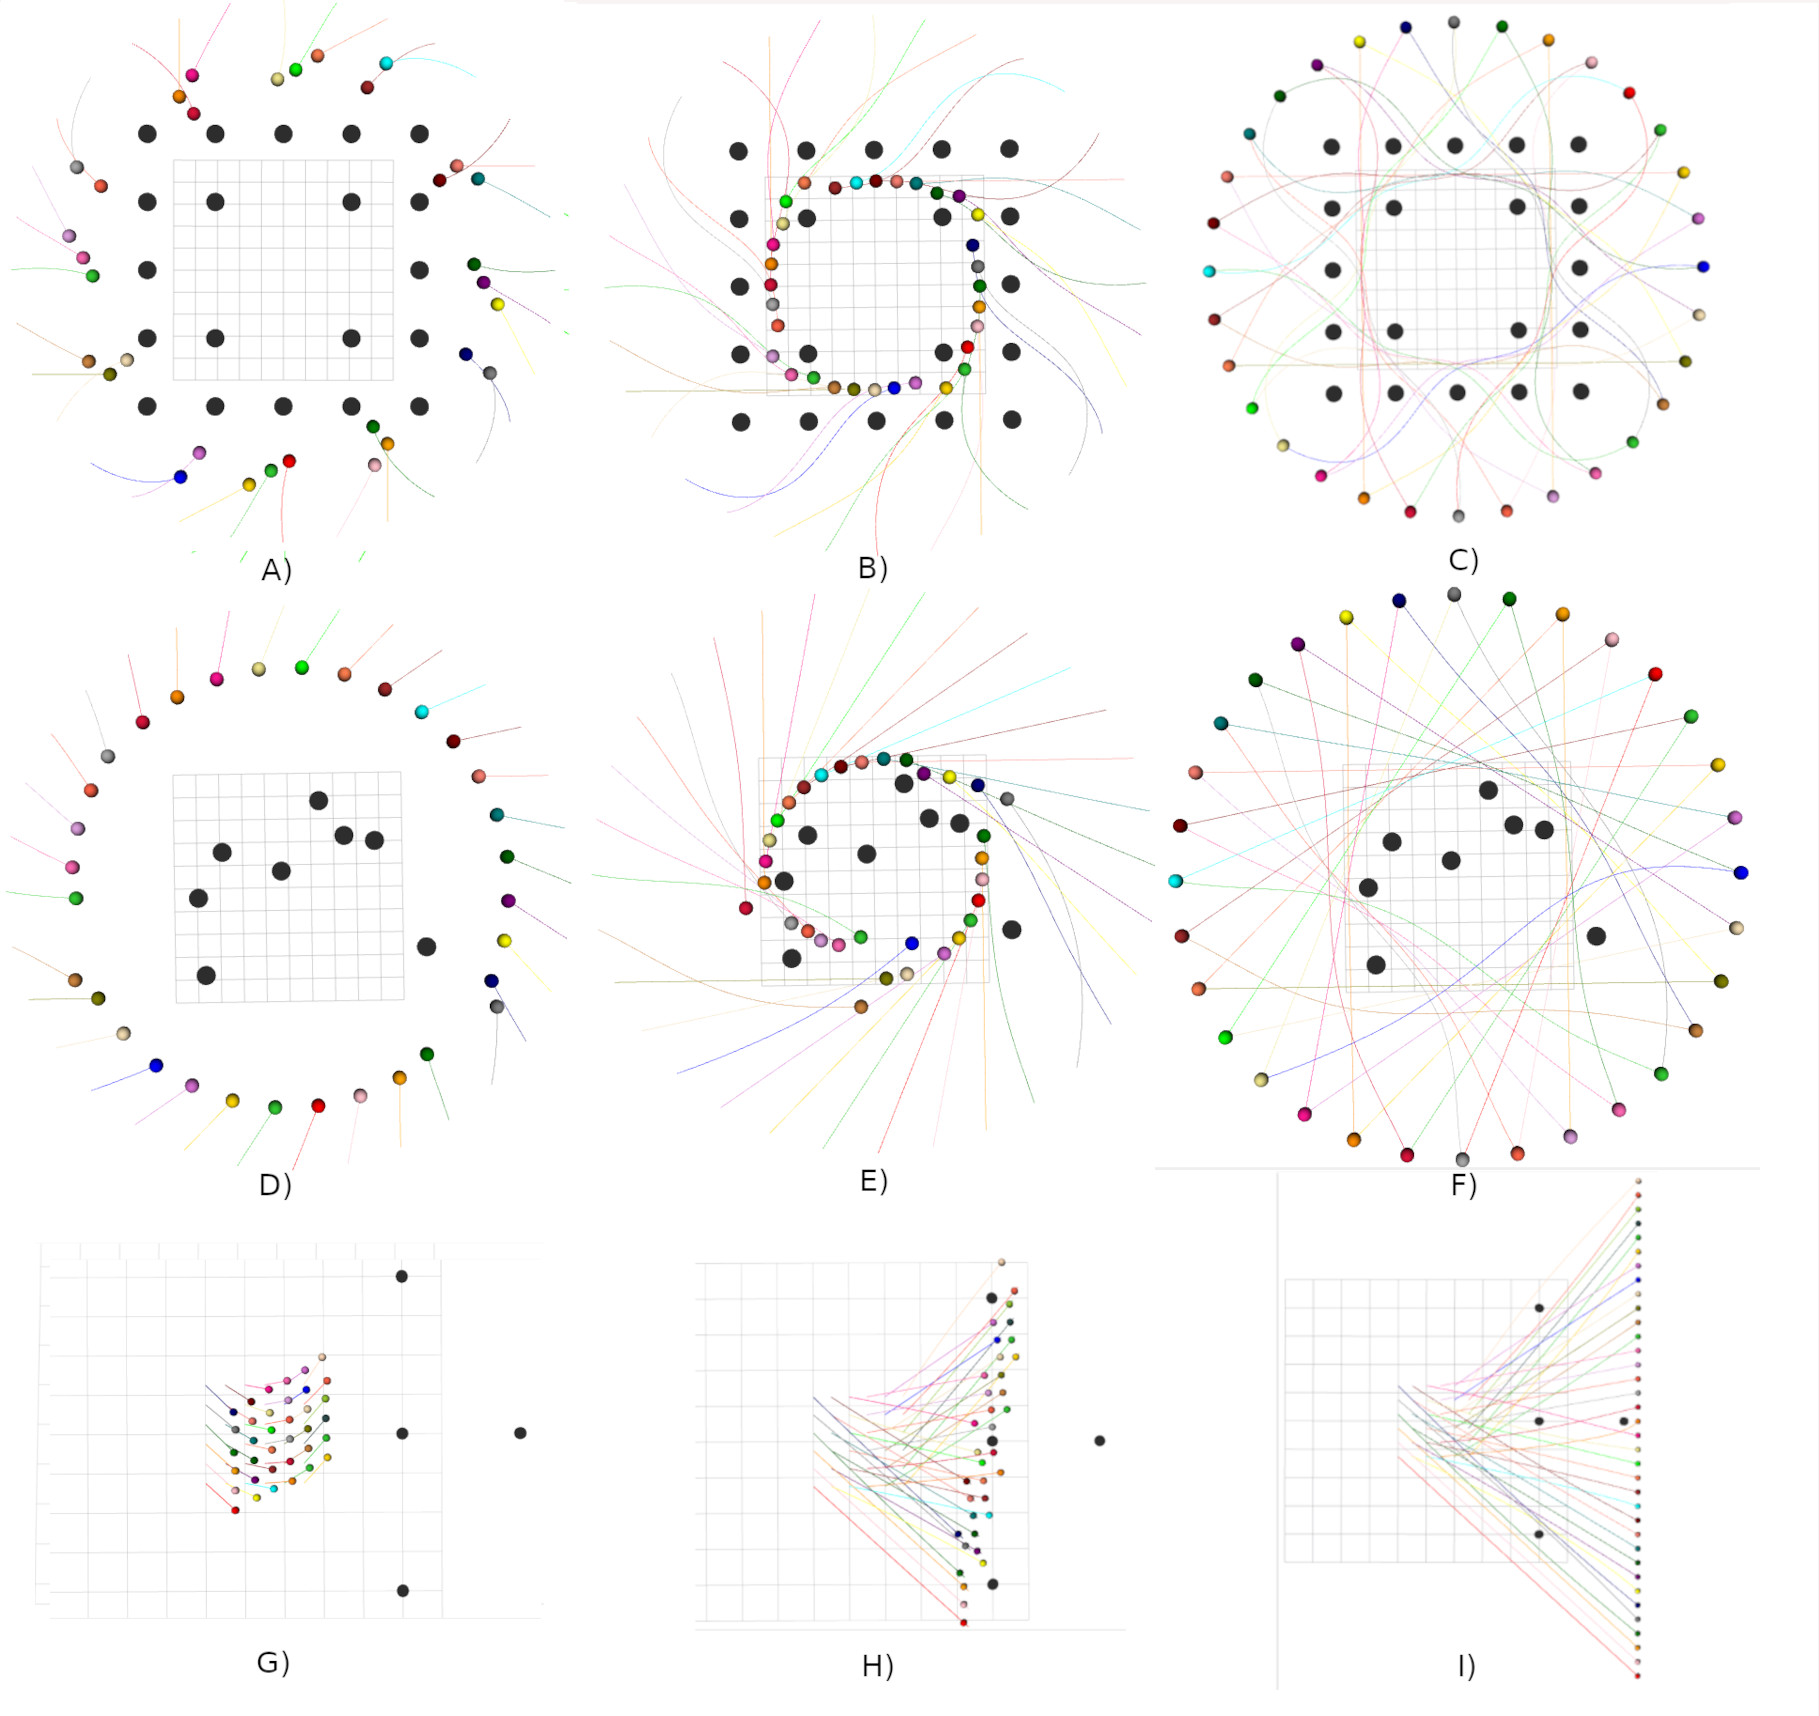
\includegraphics{figures/gpu_mat/trajectory_snapshots.jpg}} 
    \caption[Multi-robot Trajectory Snapshots]{Trajectory snapshots for (A-C) 32 robots, each of radius 0.3m arranged in a circle and 20 obstacles of radius 0.4m, (D-F) 32 robots, each of radius 0.3m arranged in a circle and 8 randomly placed obstacles of radius 0.4m, (G-I) 36 robots, each of radius 0.1m arranged in a grid configuration are required to move to a line formation. Also, the environment has 4 static obstacles, each of radius 0.15m.}
    \label{figure2}
\end{figure}

\begin{figure}
    \centering
    {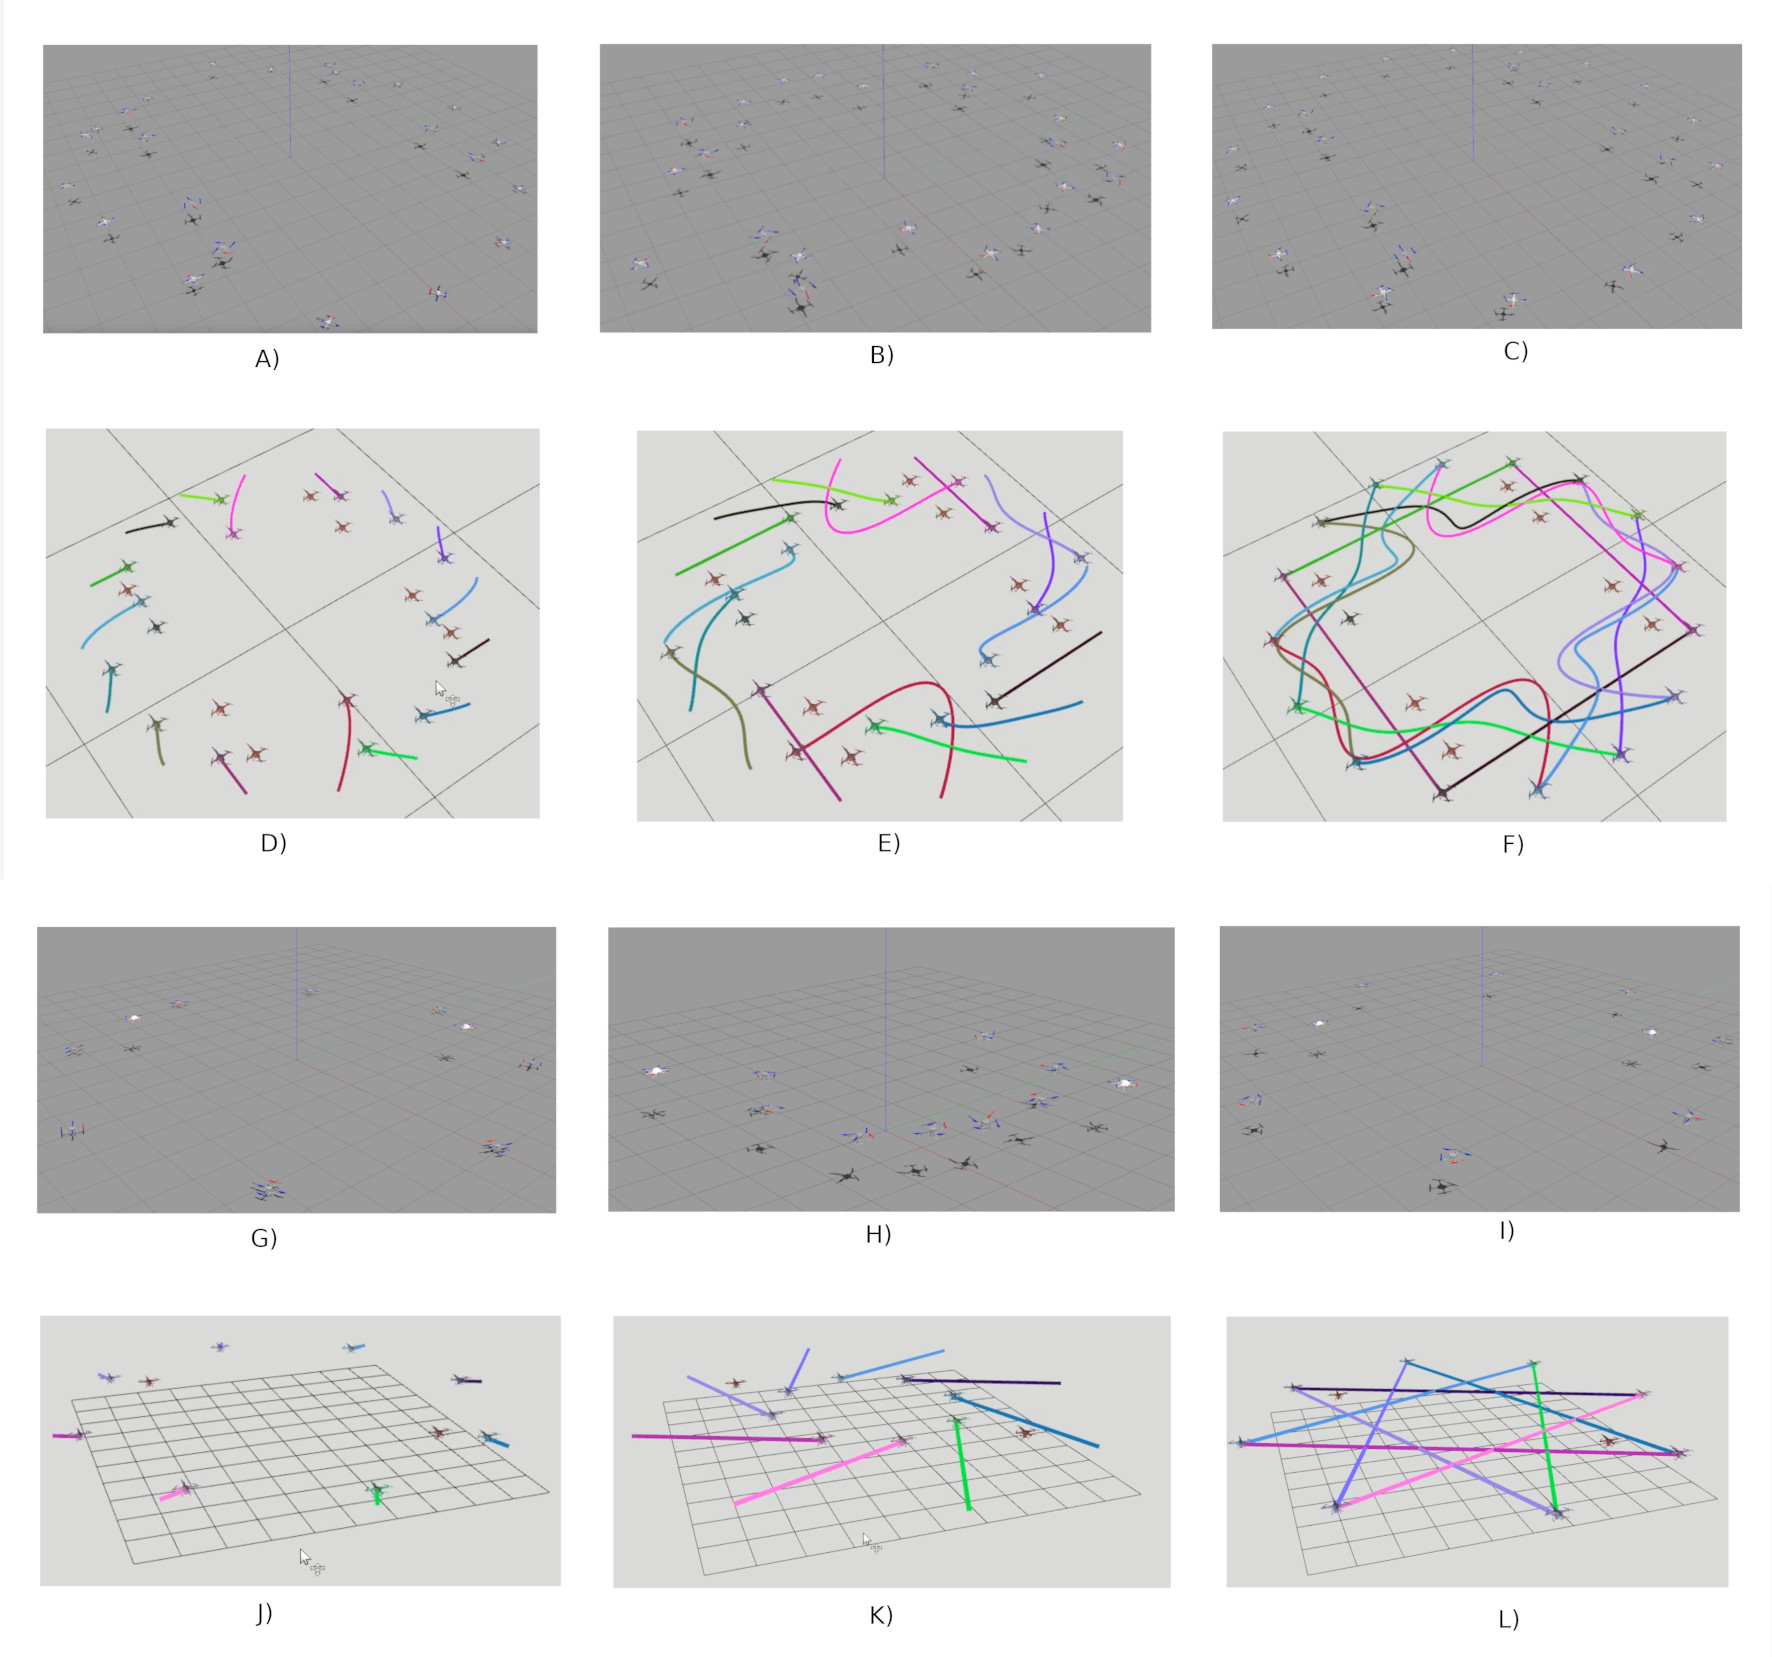
\includegraphics{figures/gpu_mat/gazebo_sim_snaps.jpg}} 
    \caption[Gazebo Simulation Snapshots]{Simulation snapshots for (A-F) 16 drones and 8 static obstacles of radius 0.3m, and (G-L) 8 drones and 2 static obstacles of radius 0.3m. (A-C) and (G-I) are screenshots of simulations on Gazebo. In (A-C), the gray static hovering drones represent static obstacles while in (G-I) white hovering drones represent static obstacles. (D-F) and (J-L) are screenshots of RViz simulations with the brown hovering drones representing static obstacles. For the full simulation videos, please refer to the following link: \url{https://www.dropbox.com/scl/fo/xnostapkvf72uudyb840t/h?dl=0&rlkey=02gjjllohbomzi0kcifbqezt9} }
    \label{figure_gazebo}
\end{figure}


A conceptually simple way of validating the convergence of the proposed optimizer is to observe the trends in residual of constraints \eqref{non_convex_equality_matrix-form} over iterations. If the residuals converge to zero, the computed trajectories are guaranteed to be collision-free. Fig. \ref{figure4} empirically provides this validation. It presents $\Vert \textbf{F}\boldsymbol{\xi}_{1, i}-\textbf{g}_i\Vert$ averaged over all $i$. Furthermore, we average the residuals over different trials in various benchmarks. We can observe from Fig.\ref{figure4} that, on average, 100 iterations are sufficient to obtain residuals around 0.01. A further increase in residuals can be obtained by increasing the number of iterations but at the expense of increasing the computation time. In our implementation, we adopt a heuristic wherein we inflate the size of the robots with four times the typical residual observed after 100 iterations.



\begin{figure}
    \centering
    {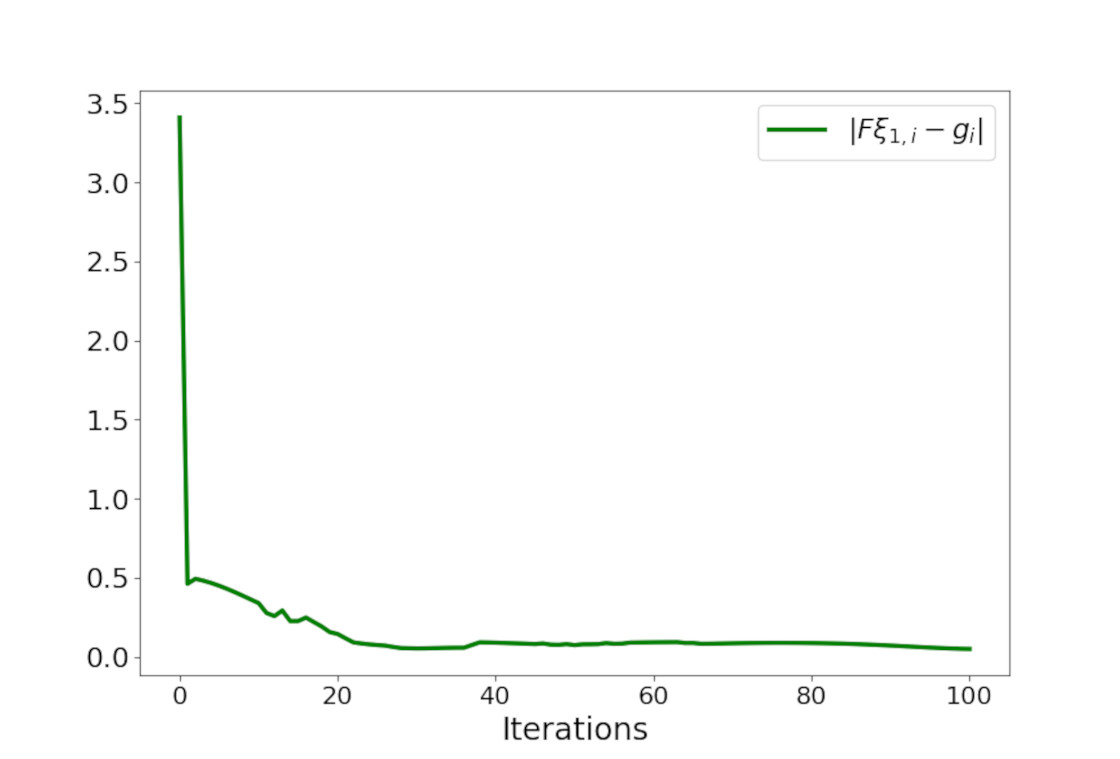
\includegraphics{figures/gpu_mat/cost_plots.jpg}} 
    \caption[GPU Optimizer Cost Plot]{Empirical validation of convergence of our optimizer. The figure shows the residual of $\Vert \textbf{F}\boldsymbol{\xi}_{1, i}-\textbf{g}_i\Vert$ averaged over all $i$ (agent index) and across different benchmarks.}
    \label{figure4}
\end{figure}

For a further sanity check, we check for inter-robot and robot-obstacle distances at each point along the computed trajectories (Fig. \ref{figure5}). Collisions are considered to have happened if the distances are less than sum of the robots' (blue line in Fig.\ref{figure5}) or robot-obstacles' (yellow line in Fig.\ref{figure5}) radii. Fig \ref{figure5} summarizes the average behavior observed across several trials, which validates the satisfaction of the collision avoidance requirement.


% shows the minimum pairwise distance between the centers of robots and obstacles for the scenarios considered in Fig \ref{figure2}. We observe that the minimum distance between any two robots always remains more than the sum of their radius, thereby guaranteeing no collision among robots. 


\begin{figure}
    \centering
    {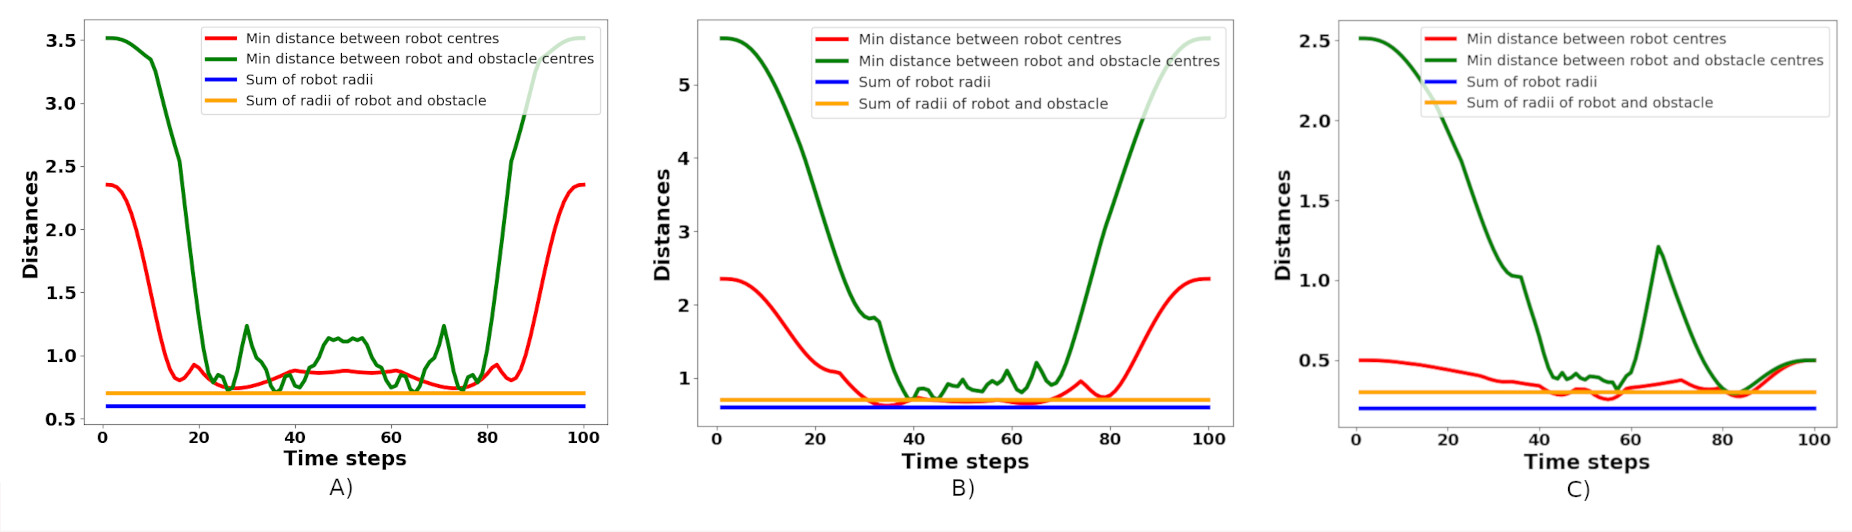
\includegraphics{figures/gpu_mat/min_distances.jpg}} 
    \caption[Minimum pairwise distances in benchmark scenes]{Figure showing the minimum of the pair-wise distances between the robots averaged across different benchmarks, some of which are shown in Fig.\ref{figure2}. The pair-wise distance is always greater than the lower bound shown in blue. Similarly, we also show the average minimum distance between the robots' and obstacles' centers. The corresponding lower bound is shown in yellow which is always respected by the computed trajectories.}
    \label{figure5}
\end{figure}


\subsection{Comparisons With State-of-the-Art}

\noindent This subsection compares our optimizer with existing state-of-the-art approaches \citep{aks_ral21} and \citep{park2020efficient}. We use the metrics Smoothness Cost, Arc-Length and Computation Time as discussed in Section \ref{sec:traj_eval_metrics}.


\subsubsection{Comparison with \citep{park2020efficient}}
Fig. \ref{figure6} presents a qualitative comparison between the trajectories obtained by our optimizer and \citep{park2020efficient} in two different benchmarks. Both approaches are successful; however, ours results in shorter trajectories. This trend is further confirmed by Fig.\ref{figure7}. Our optimizer achieves an average reduction of $3.90\%$ and $13.72\%$ in arc-length in 16 and 32 robots benchmarks, respectively. Furthermore, the performance gap between our optimizer and \citep{park2020efficient} increases as the environment becomes more cluttered with static obstacles. We also observe similar trends in the smoothness metric, with the performance gap being even starker. Our optimizer achieves an average reduction of $35.86\%$ and $59.06\%$ in smoothness cost in 16 and 32 robots benchmark, respectively.


Table \ref{table_comptime_seq} compares the computation time of our optimizer and \citep{park2020efficient}. Our optimizer shows better scaling with the number of robots and obstacles in the environment. On the considered benchmark, our optimizer shows a worst and best case improvement of $74.28 \%$ and $98.48 \%$ respectively. The trends in computation time can be understood in the following manner. The approach of \citep{park2020efficient} uses sampling-based multi-agent pathfinding algorithms to compute initial guesses for the robot trajectories. As the environment becomes more cluttered, the computational cost of computing the initial trajectories increases dramatically. Moreover, their sequential optimization also becomes increasingly more computationally intensive as the number of robots and obstacle increase. 

In contrast, our optimizer only requires matrix-matrix products, and the dimension of these matrices increases linearly with the number of robots and obstacles. This linear scaling along with GPU parallelization explains our computation time. 

\begin{figure}
    \centering
    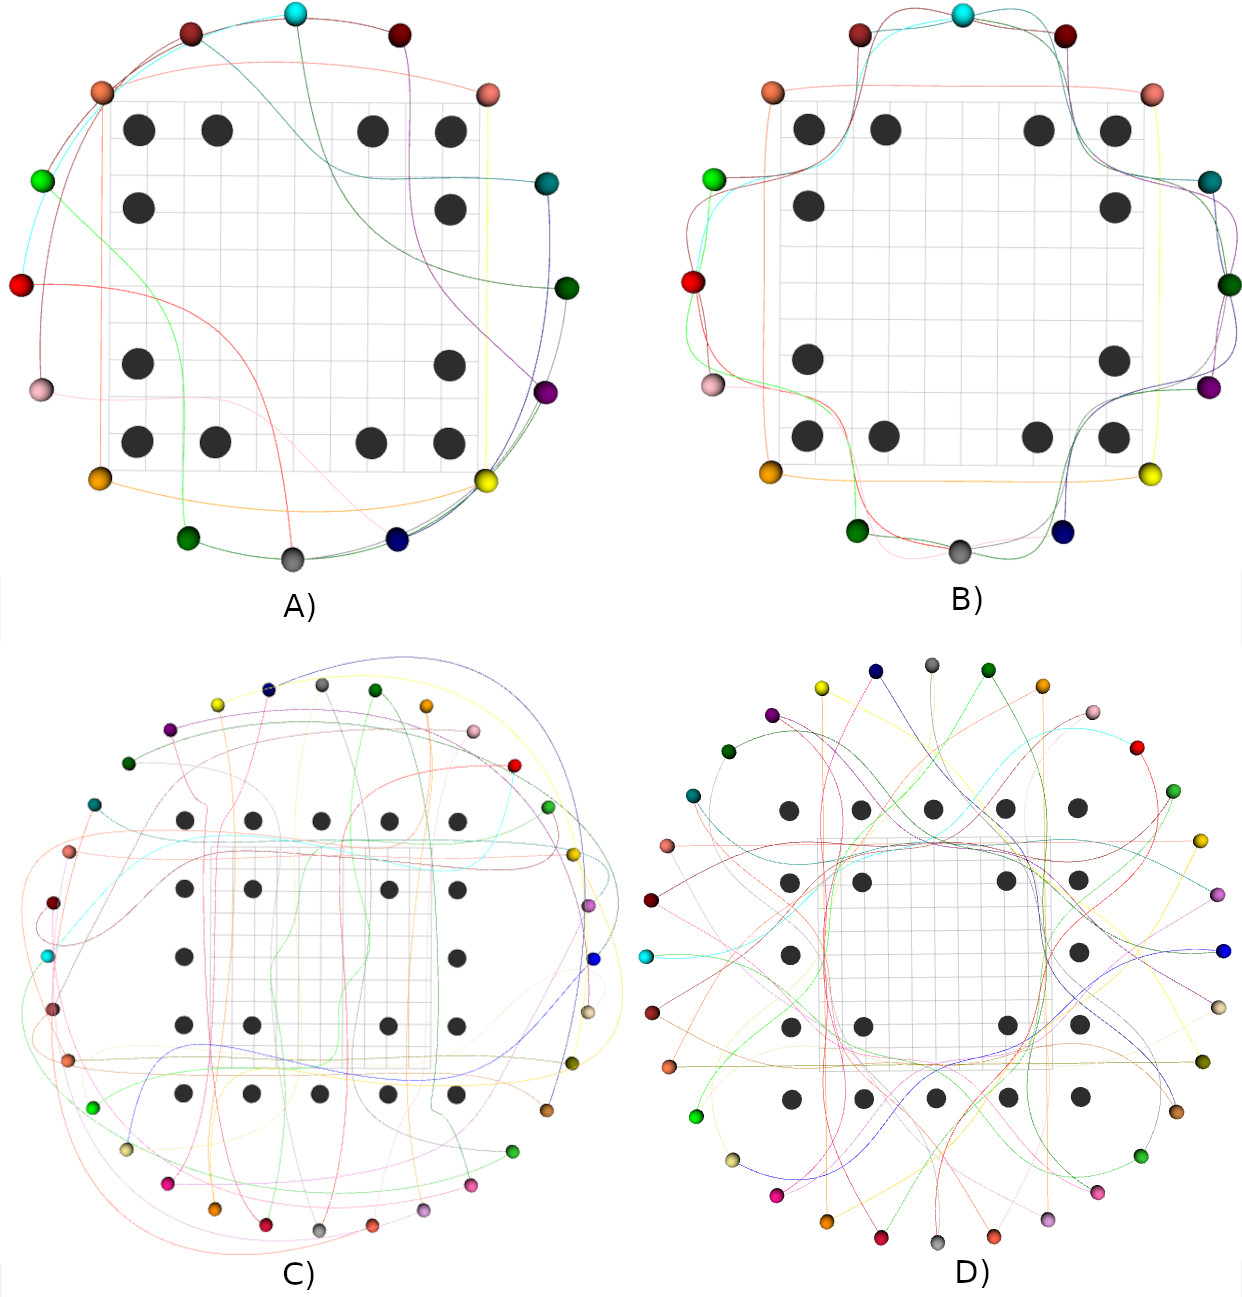
\includegraphics{figures/gpu_mat/qualitative_benchmark.jpg}
    \caption[Qualitative Benchmark against Multi-Robot State-of-the-Art]{Comparison of trajectories generated by \citep{park2020efficient}(A),C)) and our optimizer(B),D)) for 16 robots-12 obstacles (upper row) and 32 robots-20 obstacles (bottom row) benchmarks. Black spheres denote static obstacles and colored spheres denote robots. Our optimizer generates trajectories with smaller arc-length than \citep{park2020efficient}.}
    \label{figure6}
\end{figure}


\begin{figure}
    \centering
    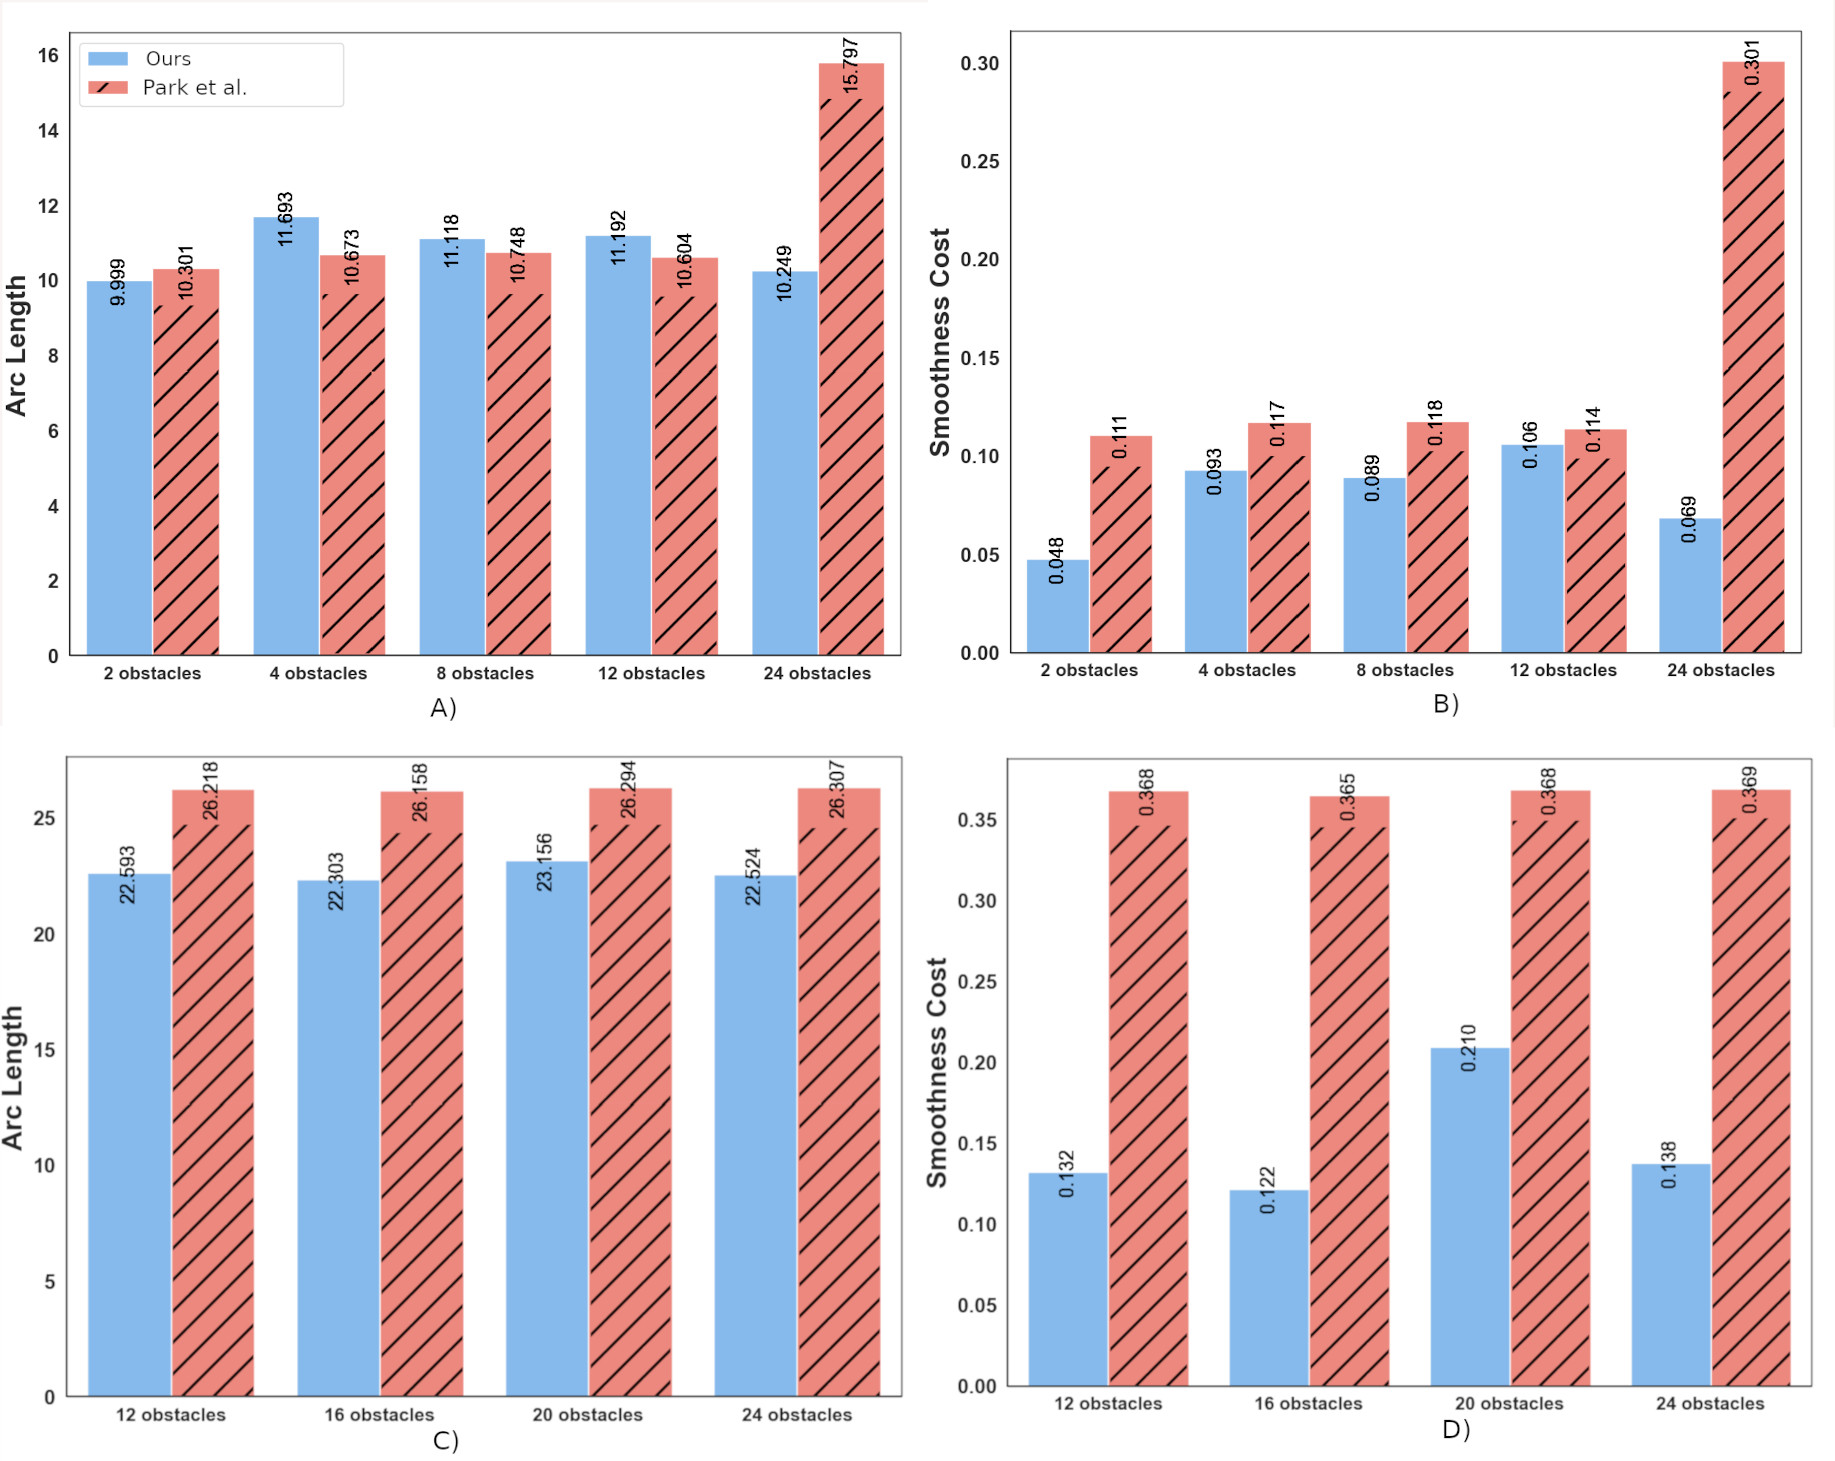
\includegraphics{figures/gpu_mat/quantitative_benchmark.jpg}
    \caption[Quantitative Benchmark against Multi-Robot State-of-the-Art]{Comparison of our optimizer with \citep{park2020efficient} in terms of arc-length and smoothness of obtained trajectories in 16 robots (A,B) and 32 robots (C,D) benchmarks. Our optimizer generates trajectories with not only better smoothness, but also with shorter arc-lengths. Moreover, the performance gap between our approach and \citep{park2020efficient} increases as the environment becomes more cluttered.}
    \label{figure7}
\end{figure}


\subsubsection{Comparison with \citep{aks_ral21}}
Table. \ref{table_3} compares the performance of our optimizer with \citep{aks_ral21}. Our core difference with \citep{aks_ral21} stems from the fact that we break a large optimization problem into smaller distributed sub-problems. In contrast, \citep{aks_ral21} retains the original larger problem itself. However, both our optimizer and  \citep{aks_ral21} use GPUs to accelerate the underlying numerical computations. Thus, unsurprisingly, \citep{aks_ral21} shows a decent scaling with the number of robots and obstacles. Nevertheless, our approach still outperforms \citep{aks_ral21}. Specifically, in 16 robot benchmarks, our optimizer shows a worst-case improvement of 2 times over \citep{aks_ral21} in computation time. As the environment becomes more cluttered, this factor increases to almost 10. In 32 robot benchmarks, the difference between our optimizer and \citep{aks_ral21}'s computation time is around nine times.

In terms of the arc-length and the smoothness metrics, our optimizer shows an improvement of around $57 \%$ and $58\%$ respectively over \citep{aks_ral21}. However, both approaches provide comparable results in the more challenging 32 robot benchmarks. The arc-length and smoothness cost difference decreases as the environment becomes more cluttered. 

\section{Discussions and Conclusion}

Joint multi-robot trajectory optimizations are generally considered intractable beyond a small number of robots. This is because the number of pair-wise collision avoidance constraints increases exponentially with the number of robots. Moreover, even the best optimization (QP) solvers show polynomial scaling with the number of constraints. We have fundamentally altered this notion through the discussion in this chapter. By employing a clever set of reformulations and parallelism offered by modern computing devices such as GPUs, we managed to compute trajectories for tens of robots in highly cluttered environments in a fraction of a second. Our formulation is simple to implement and involves computing just matrix-matrix products. Such computations can be trivially accelerated or parallelized on GPUs using off-the-shelf libraries like JAX (\cite{bradbury2020jax}). We benchmarked our approach against two strong state-of-the-art baselines and showed substantial improvement over them in terms of computation time and trajectory quality. 

Our work has potential beyond multi-robot coordination for interaction-aware trajectory prediction. We show in Appendix \ref{sec:appendix-RVO} and \ref{sec:appendix-MAPF} how our multiagent optimizer may be used to improve the quality of trajectories obtained from multi-agent collision avoidance methods, such as Reciprocal Velocity Obstacle(RVO)\cite{RVO} and Multi-Agent Pathfinding(MAPF)\cite{sharon_journal}. We recognize that our optimizer's current form is suited for only holonomic robots and that our optimizer can be extended in the future to non-holonomic constraints for the coordination of car-like vehicles. 

%%%%%%%%%%%%%%%putting 1 line empty

\begin{table}
\centering
\caption{Important Symbols used in our optimizer} \label{table_1}
\scriptsize
\begin{tabular}{|p{3cm}|p{7cm}|p{7cm}|}\hline
\mbox{$n_{p}$, $n_{v}$, $n_{r}$}  & Planning steps, number of variables parameterizing trajectory along each motion axis, and number of robots, respectively.
\\ \hline
\mbox{ $a, b $} & Spheroid dimensions
\\ \hline
\mbox{$x_i(t), y_i(t), z_i(t)$} & 
 Position of $i^{th}$ robot at time $t$.
\\ \hline
\mbox{$\overline{x}_i(t), \overline{y}_i(t), \overline{z}_i(t)$} & Predicted position of $j^{th}$ agent.
\\ \hline
\mbox{$\boldsymbol{\lambda}_{i}$}
 &  Lagrangian multiplier 
\\ \hline
\end{tabular}
\normalsize
\vspace{-0.7cm}
\end{table}


%%%%%%%%%%%%%%%%%%%%%%one line empty

%%%%%%%%%%%%%%%%%%%% one line empty 

\begin{table}
\begin{center}
\caption{Comparison with current state-of-the-art \citep{park2020efficient} in terms of computation time.  }
\label{table_comptime_seq}
\begin{tabular}{ |p{3.5cm}|p{3cm}|p{2cm}|p{2cm}|}
\hline
 Number of robots & Number of Obstacles & ours[s] & \citep{park2020efficient}[s]  \\
 \hline
 32 & 24 & 0.21 &  12.897\\
 \hline
 32 & 20 &  0.20 &  11.827\\
 \hline
 32 & 16 & 0.20 & 12.423\\
 \hline
 32 & 12 & 0.19 & 12.504\\
 \hline
 16 & 24 & 0.17 & 0.795\\ 
 \hline
 16 & 12 & 0.17& 0.661\\
 \hline
 16 & 8 & 0.16& 0.680\\
 \hline
 16 & 4 & 0.16 & 0.702\\
 \hline
 16 & 2 & 0.15 & 0.621\\
 \hline
\end{tabular}
\end{center}
\end{table}

%%%%%%%%%%%%%%%%%%%%%%%%%%%%%%%%%%%%%%%%%%%%
%%%%%%%%%%%%%%%%%%%%%%%% one line empty 

\begin{table}
\centering
\caption{ Comparison with \citep{aks_ral21} in terms of computation time, arc-length and smoothness cost }
\label{table_3}
\scriptsize
\begin{tabular}{|p{2cm}|p{2.5cm}|p{3.5cm}|p{2cm}|p{2cm}|p{2cm}|}
\hline
Number of robots & Number of Obstacles &Benchmark & Computation time[s] & Arc-length[M] & Smoothness cost  \\ 
\hline
 \multirow{2}{*}{}&2  & \citep{aks_ral21}  &  0.34 & 13.488 & 0.102\\  
 \cline{2-6} 
 \multirow{2}{*}{}&2  & Ours &  0.15  &  9.999 & 0.048\\  
 \cline{2-6}
 \multirow{2}{*}{16 robot}& 4 & \citep{aks_ral21} & 0.37 & 14.257& 0.114\\
 \cline{2-6}
  \multirow{2}{*}{}& 4 & Ours  & 0.16 & 11.693& 0.093\\
 \cline{2-6}
 \multirow{2}{*}{}&8 & \citep{aks_ral21} & 0.70 &15.539 & 0.140\\
 \cline{2-6}
  \multirow{2}{*}{}&8 & Ours & 0.16 &11.118 & 0.089\\
 \cline{2-6}
 \multirow{2}{*}{}&12 & \citep{aks_ral21}  & 0.79 & 15.931 & 0.159\\
  \cline{2-6}
\multirow{2}{*}{} & 12  & Ours & 0.17 & 11.192 & 0.106\\ 
\cline{2-6}
 \multirow{2}{*}{}&24 & \citep{aks_ral21}  &1.49  & 24.198 & 0.164\\
  \cline{2-6}
\multirow{2}{*}{} & 24  & Ours & 0.17 & 10.249 & 0.069\\ 
\hline \hline
\multirow{2}{*}{} & 12  & \citep{aks_ral21} & 1.688 & 23.855  &0.157\\
\cline{2-6}
\multirow{2}{*}{} & 12  & Ours & 0.19 & 22.593 & 0.132\\
\cline{2-6}
\multirow{2}{*}{} & 16  & \citep{aks_ral21} & 1.752 &24.04 &0.164\\
\cline{2-6}
\multirow{2}{*}{32 robots} & 16  & Ours & 0.20 & 22.303 &0.122 \\
\cline{2-6}
\multirow{2}{*}{} & 20 & \citep{aks_ral21} & 1.804  &24.14 &0.170\\
\cline{2-6}
\multirow{2}{*}{} & 20  & Ours & 0.20 & 23.156 &0.210 \\
\cline{2-6}
\hline
\end{tabular}
\normalsize
\end{table}

%%%%%%%%%%%%%%%%%%%%%one line empty

% \section{\label{sec:abstract}Abstract}

% Near-term quantum hardware can support two-qubit operations only on the qubits that can interact with each other. Therefore, to execute an arbitrary quantum circuit on the hardware, compilers have to first perform the task of qubit routing, i.e., to transform the quantum circuit either by inserting additional SWAP gates or by reversing existing CNOT gates to satisfy the connectivity constraints of the target topology.  The depth of the transformed quantum circuits is minimized by utilizing the Monte Carlo tree search (MCTS) to perform qubit routing by making it both construct each action and search over the space of all actions. It is aided in performing these tasks by a Graph neural network that evaluates the value function and action probabilities for each state. Along with this, we propose a new method of adding mutex-lock like variables in our state representation which helps factor in the parallelization of the scheduled operations, thereby pruning the depth of the output circuit. Overall, our procedure (referred to as QRoute) performs qubit routing in a hardware agnostic manner, and it outperforms other available qubit routing implementations on various circuit benchmarks.

% {\smaller (Published in the Proceedings of AAAI Conferenence on Artificial Intelligence, 2022 \cite{self-qroute})}    
% %\tableofcontents

% \section{\label{sec:intro}Introduction}

% The present-day quantum computers, more generally known as Noisy Intermediate-Scale quantum (NISQ) devices \cite{nisq_preskill} come in a variety of hardware architectures \cite{IBMQ, hardware_sycamore, hardware_rigetti_aspen, hardware_xanadu}, but there exist a few problems pervading across all of them. These problems constitute the poor quality of qubits, limited connectivity between qubits, and the absence of error-correction for noise-induced errors encountered during the execution of gate operations. These place a considerable restriction on the number of instructions that can be executed to perform useful quantum computation \cite{nisq_preskill}. Collectively these instructions can be realized as a sequential series of one or two-qubit gates that can be visualized more easily as a quantum circuit as shown in Fig. \ref{fig:orig_circ} \cite{others_childs}.

% To execute an arbitrarily given quantum circuit on the target quantum hardware, a compiler routine must transform it to satisfy the connectivity constraints of the topology of the hardware \cite{qroute_tket}. These transformations usually include the addition of SWAP gates and the reversal of existing CNOT gates. This ensures that any non-local quantum operations are performed only between the qubits that are nearest-neighbors. This process of circuit transformation by a compiler routine for the target hardware is known as qubit routing \cite{qroute_tket}. The output instructions in the transformed quantum circuit should follow the connectivity constraints and essentially result in the same overall unitary evolution as the original circuit \cite{qroute_dqn2}.

% In the context of NISQ hardware, this procedure is of extreme importance as the transformed circuit will, in general, have higher depth due to the insertion of extra SWAP gates. This overhead in the circuit depth becomes more prominent due to the high decoherence rates of the qubits and it becomes essential to find the most optimal and efficient strategy to minimize it \cite{qroute_tket, qroute_dqn1, qroute_dqn2}. In this chapter, we present a procedure that we refer to as \textit{QRoute}. We use Monte Carlo tree search (MCTS), which is a look-ahead search algorithm for finding optimal decisions in the decision space guided by a heuristic evaluation function \cite{mcts_bandit_1, mcts_bandit_2, mcts_uct}. We use it for explicitly searching the decision space for depth minimization and as a stable and performant machine learning setting. It is aided by a Graph neural network (GNN) \cite{nn_edge_conv}, with an architecture that is used to learn and evaluate the heuristic function that will help guide the MCTS.

% %\textit{Structure}: In Section \ref{sec:qubit-routing}, we introduce the problem of qubit routing, the previous works that are done in the field, and show how our work differs from them. The methodology of the QRoute algorithm is described in Section \ref{sec:method}. In Section \ref{sec:results}, we benchmark the performance of our algorithm against other state-of-the-art quantum compilers. Finally, we discuss our results and  possible improvements in Section \ref{sec:discussion-conclusion}.

% \begin{figure}
%     \centering
%     \hfill
%     \begin{subfigure}[b]{0.30\linewidth}
%         \includegraphics[width=\textwidth]{figures/qroute/orig_circ.pdf}
%         \caption{Quantum circuit\label{fig:orig_circ}}
%     \end{subfigure}
%     \hfill
%     \begin{subfigure}[b]{0.30\linewidth}
%         \includegraphics[width=0.85\textwidth]{figures/qroute/sliced_circ.pdf}
%         \caption{Decomposed circuit\label{fig:sliced_circ}}
%     \end{subfigure}
%     \hfill
%     \begin{subfigure}[b]{0.35\linewidth}
%         \includegraphics[width=\textwidth]{figures/qroute/transformed_circ.pdf}
%         \caption{Decomposed transformed circuit\label{fig:transformed_circ}}
%     \end{subfigure}
%     \hfill
%     \caption[Topologies of Quantum Computing hardware qRoute is tested on]{An example of qubit routing on a quantum circuit for 3$\times$3 grid architecture (Figure \ref{fig:3-3-arch}). (a) For simplicity, the original quantum circuit consists only of two-qubit gate operations. (b) Decomposition of the original quantum circuit into series of slices such that all the instructions present in a slice can be executed in parallel. The two-qubit gate operations: $\{d,e\}$ (green) comply with the topology of the grid architecture whereas the operations: $\{a, b, c, f\}$ (red) do not comply with the topology (and therefore cannot be performed). Note that the successive two-qubit gate operations on $q_3\rightarrow q_4$ (blue) are redundant and are not considered while routing. (c) Decomposition of the transformed quantum circuit we get after qubit routing. Four additional SWAP gates are added that increased the circuit depth to $5$, i.e., an overhead circuit depth of $2$. The final qubit labels are represented at the end right side of the circuit. The qubits that are not moved (or swapped) are shown in brown ($\{q_1, q_5\}$), while the rest of them are shown in blue.}
%     %Note that the overall unitary operation performed by the circuit is preserved despite the changes in the order of two-qubit gate operations.}
%     \label{fig:routing-example}
% \end{figure}

% \begin{figure}
%     \centering
%     \begin{subfigure}[b]{0.4\linewidth}
%         \centering
%         \includegraphics[width=0.5\linewidth]{figures/qroute/Grid-device.pdf}
%         \caption{3$\times$3 grid architecture with edges (i.e. neighboring qubits) labelled \label{fig:3-3-arch}}
%     \end{subfigure}
%     \begin{subfigure}[b]{0.5\linewidth}
%         \centering
%         \includegraphics[width=0.5\linewidth]{figures/qroute/QX20-device.pdf}
%         \caption{IBMQX-20 architecture represented as a graph}
%     \end{subfigure}
%     \caption{Examples of qubit connectivity graphs for some common quantum architectures}
%     \label{fig:topology-example}
% \end{figure}

% \section{\label{sec:qubit-routing}Qubit Routing}
% In this section, we begin by defining the problem of qubit routing formally and discussing the work done previously in the field.

% \subsection{\label{sec:intro-defn}Describing the Problem}
% The topology of quantum hardware can be visualized as a qubit connectivity graph (Fig. \ref{fig:topology-example}). Each node in this graph would correspond to a physical qubit which in turn might correspond to a logical qubit. The quantum instruction set, which is also referred to as quantum circuit (Fig. \ref{fig:orig_circ}), is a sequential series of single-qubit and two-qubit gate operations that act on the logical qubits. The two-qubit gates such as CNOT can only be performed between two logical qubits iff there exists an edge between the nodes that correspond to the physical qubits, \cite{qroute_dqn1}. This edge could be either unidirectional or bidirectional, i.e., CNOT can be performed either in one direction or in both directions. In this work, we consider only the bidirectional case, while noting that the direction of a CNOT gate can be reversed by sandwiching it between a pair of Hadamard gates acting on both control and target qubits \cite{utk_equiv_circuits}. 

% Given a target hardware topology $\mathcal{D}$ and a quantum circuit $\mathcal{C}$, the task of qubit routing refers to transforming this quantum circuit by adding a series of SWAP gates such that all its gate operations then satisfy the connectivity constraints of the target topology (Fig. \ref{fig:transformed_circ}). Formally, for a routing algorithm $\textrm{R}$, we can represent this process as follows:
% \begin{equation}
% \textrm{R}(\mathcal{C},\ \mathcal{D}) \rightarrow \mathcal{C}^{\prime}
% \end{equation}
% Depth of $\mathcal{C}^{\prime}$ (transformed quantum circuit) will, in general, be more than that of the original circuit due to the insertion of additional SWAP gates. This comes from the definition of the term \textit{depth} in the context of quantum circuits. This can be understood by decomposing a quantum circuit into series of individual slices, each of which contains a group of gate operations that have no overlapping qubits, i.e., all the instructions present in a slice can be executed in parallel (Fig. \ref{fig:sliced_circ}). The depth of the quantum circuit then refers to the minimum number of such slices the circuit can be decomposed into, i.e., the minimum amount of parallel executions needed to execute the circuit. The goal is to minimize the overhead depth of the transformed circuit with respect to the original circuit.

% This goal involves solving two subsequent problems of (i) qubit allocation, which refers to the mapping of program qubits to logic qubits, and (ii) qubit movement, which refers to routing qubits between different locations such that interaction can be made possible \cite{utk_qubit_noise}. In this work, we focus on the latter problem of qubit movement only and refer to it as qubit routing. However, it should be  noted that qubit allocation is also an important problem and it can play an important role in minimizing the effort needed to perform qubit movement.



% \subsection{\label{sec:intro-related}Related Work}

% The first major attraction for solving the qubit routing problem was the competition organized by IBM in 2018 to find the best routing algorithm. This competition was won by \cite{zulehner2018mapping}, for developing a Computer Aided Design-based (CAD) routing strategy. Since then, this problem has been presented in many different ways. These include graph-based architecture-agnostic solution by \cite{qroute_tket}, showing equivalence to the travelling salesman problem by \cite{paler_torus}, machine learning based methods by \cite{paler_ml}, and heuristic approaches by \cite{review-1}, \cite{review-2}, \cite{review-3}, etc. A reinforcement learning in a combinatorial action space solution was proposed by \cite{qroute_dqn1}, which suggested used simulated annealing to search through the combinatorial action space, aided by a Feed-Forward neural network to judge the long-term expected depth. This was further extended to use Double Deep Q-learning and prioritized experience replay by \cite{qroute_dqn2}. 

% Recently, Monte Carlo tree search (MCTS), a popular reinforcement learning algorithm \cite{mcts_survey} previously proven successful in a variety of domains like playing puzzle games such as Chess and Go \cite{mcts_alphago}, and was used by \cite{qroute_mcts} to develop a qubit routing solution. 
% %However, they used MCTS in the context of minimizing the total volume of quantum circuits (i.e., the number of gates ignoring the parallelization).

% % \begin{figure*}[t]
% %     \includegraphics[width=\linewidth]{figures/qroute/Evolution.pdf}
% % 	\caption{\label{fig:routing-progress}Routing progress for 3$\times$3 grid architecture while for the quantum circuit in Fig. \ref{fig:orig_circ}. Initial state shows the gate scheduled on each qubit which gets executed as control and target qubit adjacent to each other via SWAPs (shown in green and purple). The final state (at time=$5$) shows the final evolved qubit mapping. Here, each state (at time step=$t$) corresponds to the $t^{\rm{th}}$ time slice in Fig. \ref{fig:transformed_circ}}
% % \end{figure*}

% \subsection{\label{sec:intro-contribution}Our Contributions}

% Our work demonstrates the use of MCTS on the task of Qubit Routing and presents state of the art results. Following are the novelties of this approach:

% \begin{itemize}
%     \item We use an array of mutex locks to represent the current state of parallelization, helping to reduce the depth of the circuits instead of the total quantum volume, in contrast to previous use of MCTS for qubit routing in \cite{qroute_mcts}.
%     \item The actions in each timestep (layer of the output circuit) belong to a innumerably large action space. We phrase the construction of such actions as a Markov decision process, making the training stabler and the results better, particularly at larger circuit sizes, than those obtained by performing simulated annealing to search in such action spaces \cite{qroute_dqn1, qroute_dqn2}. Such approach should be applicable to other problems of a similar nature.
%     \item Graph neural networks are used as an improved architecture to help guide the tree search.
% \end{itemize}

% Finally, we provide a simple python package containing the implementation of QRoute, together with  an easy interface for trying out different neural net architectures, combining algorithms, reward structures, etc.

% \begin{figure}[ht]
%     \centering
%     \includegraphics[width=\linewidth]{figures/qroute/Search.pdf}
%     \caption[Visualization of steps in Monte Carlo Tree Search]{
%         Iteration of a Monte Carlo tree search: (i) select - recursively choosing a node in the search tree for exploration using a selection criteria, (ii) expand - expanding the tree using the available actions if an unexplored leaf node is selected, (iii) rollout - estimating long term reward using a neural network for the action-state pair for the new node added to search tree, and (iv) backup - propagating reward value from the leaf nodes upwards to update the evaluations of its ancestors.}
%     \label{fig:mcts-explainer}
% \end{figure}


% \newtheorem{defn}{Definition}[section]

% \section{\label{sec:method}Method}

% The QRoute algorithm takes in an input circuit and an injective map, $\mathcal{M}: Q \rightarrow N$, from logical qubits to nodes (physical qubits). Iteratively, over multiple timesteps, it tries to schedule the gate operations that are present in the input circuit onto the target hardware. To do so, from the set of unscheduled gate operations, $\mathcal{P}$, it takes all the current operations, which are the first unscheduled operation for both the qubits that they act on, and tries to make them into local operations, which are those two-qubit operations that involve qubits that are mapped to nodes connected on the target hardware.

% In every timestep $t$, QRoute starts by greedily scheduling all the operations that are both current and local in $\mathcal{P}$. To evolve $\mathcal{M}$, it then performs a Monte Carlo tree search (MCTS) to find an optimal set of SWAPs by the evaluation metrics described in the Section \ref{sec:method-mcts} such that all operations in the current timestep put together form a parallelizable set, i.e., a set of local operations such that no two operations in the set act on the same qubit. The number of states we can encounter in the action space explodes exponentially with the depth of our search, therefore an explicit search till the circuit is done compiling is not possible. Therefore we cut short our search at some shallow intermediate state, and use a neural network to get its heuristic evaluation. Detailed algorithm has been presented in appendix \ref{appendix:mcts}.


% The following subsections describe in greater detail the working of the search and the heuristic evaluation.

% \subsection{\label{sec:method-state} State and Action Space}

% \begin{defn}[State]
%     It captures entire specification of the state of compilation at some timestep t. Abstractly, it is described as:
%     \begin{equation}
%         s_{t} = (\mathcal{D}, \ \mathcal{M}_{t},\ \mathcal{P}_{t},\ \mathcal{L}_{t})
%     \end{equation}

%     where, $\mathcal{D}$ is the topology of target hardware, and $\mathcal{M}_t$ and $\mathcal{P}_t$ represents the current values of $\mathcal{M}$ and $\mathcal{P}$ respectively. $\mathcal{L}_{t}$ is the set of nodes that are locked by the gate operations from the previous timestep and therefore cannot be operated in the current timestep. 
% \end{defn}


% \begin{defn}[Action]
%     It is a set of SWAP gates (represented by the pair of qubits it acts on) such that all gates are local, and its union with the set of operations that were scheduled in the same timestep forms a parallelizable set.
% \end{defn}

% We are performing a tree search over state-action pairs. Since the number of actions that can be taken at any timestep is exponential in the number of connections on the hardware, we are forced to build a single action up, step-by-step. 

% \begin{defn}[Move]
%     It is a single step in a search procedure which either builds up the action or applies it to the current state. Moves are of the following two types:
%     \begin{enumerate}
%         \item SWAP($n_1$, $n_2$): Inserts a new SWAP on nodes $n_1$ and $n_2$ into the action set. Such an insertion is only possible if the operation is local and resulting set of operations for the timestep form a parallel set.
%         \item COMMIT: Finishes the construction of the action set for that timestep. It also uses the action formed until now to update the state $s_t$ (schedules the SWAP gates on the hardware), and resets the action set for the next step.
%     \end{enumerate}
% \end{defn}

% In reality, different gate operations take different counts of timesteps for execution. For example, if a hardware requires SWAP gate to be broken down into CNOT gates, then it would take three timesteps for complete execution \cite{utk_equiv_circuits}. This means, operations which are being scheduled must maintain mutual exclusivity with other other operations over the nodes which participates in them. This is essential to minimizing the depth of the circuit since it models paralleizability of operations.

% However, constructing a parallelizable set and representing the state of parallelization to our heuristic evaluator is a challenge. But an analogy can be drawn here to the nodes being thought of as ``resources" that cannot be shared, and the operations as ``consumers" \cite{mutex_dijkstra}. This motivates us to propose the use of Mutex Locks for this purpose. These will lock a node until a scheduled gate operation involving that node executes completely. Therefore, this allows our framework to naturally handle different types of operations which take different amounts of time to complete.

% % On some hardware, SWAP gates are not primitive and get decomposed to three CNOT gates. Therefore they are thrice as slow as other primitive gates. This is easily modelled by keeping the mutex locks for those nodes locked for three timesteps. Therefore, this allows our framework to naturally handle different types of operations which take different amounts of time to complete.

% For every state-action pair, the application of a feasible move $m$ on it will result in a new state-action pair: $(s,a) \xrightarrow[]{m} (s^\prime,a^\prime)$. This is a formulation of the problem of search as a Markov Decision Process. Associated with each such state-action-move tuple $((s, a), m)$, we maintain two additional values that are used by MCTS:

% \begin{enumerate}
% \item \textit{N-value} - The number of times we have taken the said move $m$ from said state-action pair $(s,a)$.
% \item \textit{Q-value} - Given a reward function $\mathcal{R}$, it is the average long-term reward expected after taking said move $m$ over all iterations of the search. (Future rewards are discounted by a factor $\gamma$)

% \begin{equation}
% \begin{split}
%     Q((s,a), m) =&\ \mathcal{R}((s,a), m)\ + \\ & \gamma \frac{\sum_{m^\prime} N((s^\prime, a^\prime), m^\prime) \cdot Q((s^\prime, a^\prime), m^\prime)}{\sum_{m^\prime} N((s^\prime, a^\prime), m^\prime)}
% \end{split}
% \end{equation}

% \end{enumerate}

% \begin{figure*}[th]
% \centering
%     \includegraphics[width=\textwidth]{figures/qroute/Architecture.pdf}
%     \caption[Graph neural network architecture that approximates value and policy function]{\label{fig:network-architecture}
%      Graph neural network architecture that approximates the value function and the policy function.}
%      %The $state$ object (orange), shown on the far left, is provided as an input. The edge convolution block (yellow) extracts the features from the input object, collects them, flattens them, and concatenates them with the rest of the input for further processing. Here, the network diverges into two segments, one called the value head, which gives a scalar output representing the quality of the state, and another policy head, which provides the probability distribution over the best action from this state.}
% \end{figure*}

% \subsection{\label{sec:method-mcts} Monte Carlo Tree Search}

% Monte Carlo tree search progresses iteratively by executing its four phases: select, expand, rollout, and backup as illustrated in Fig. \ref{fig:mcts-explainer}. In each iteration, it begins traversing down the existing search tree by selecting the node with the maximum UCT value (Eq. \ref{eq:uct}) at each level. During this traversal, whenever it encounters a leaf node, it expands the tree by choosing a move $m$ from that leaf node. Then, it estimates the scalar evaluation for the new state-action pair and backpropagates it up the tree to update evaluations of its ancestors.

% To build an optimal action set, we would want to select the move $m$ with the maximum true Q-value. But since true Q-values are intractably expensive to compute, we can only approximate the Q-values through efficient exploration. We use the Upper Confidence Bound on Trees (UCT) objective \cite{mcts_uct} to balance exploration and exploitation as we traverse through the search tree. Moreover, as this problem results in a highly asymmetric tree, since some move block a lot of other moves, while others block fewer moves, we use the formulation of UCT adapted for asymmetric trees \cite{mcts_assymetric}:

% \begin{equation}\label{eq:uct}
% \begin{split}
%     \textrm{UCT}((s,a), m) =&\ Q((s,a), m)\ + \\ & c \frac{\sqrt{\sum_m N((s,a), m)}}{N((s,a), m)} \times p(m \vert (s,a))
% \end{split}
% \end{equation}

% Here, the value $p(m | (s,a))$ is the prior policy function, which is obtained by adding a Dirichlet noise to the policy output of the neural network \cite{mcts_alphazero}. As MCTS continues probing the action space, it gets a better estimate of the true values of the actions. This means that it acts as a policy enhancement function whose output policy (Eq. \ref{eq:mcts_output}) can be used to train the neural network's prior ($\pi$), and the average Q-value computed can be used to train its scalar evaluation (Eq. \ref{eq:train_nn}).

% \begin{equation}\label{eq:mcts_output}
%     \pi(m | (s,a)) \propto N((s, a), m))
% \end{equation}

% \begin{equation}\label{eq:train_nn}
%     \mathcal{V}((s,a)) = \frac{\sum_{m} Q((s,a), m)}{\sum_{m} N((s,a), m)}
% \end{equation}



% The details of how MCTS progresses have been elaborated in the supplementary. Once it gets terminated, i.e., the search gets completed, we go down the tree selecting the child with the maximum Q-value at each step until a COMMIT action is found, we use the action set of the selected state-action pair to schedule SWAPs for the current timestep, and we re-root the tree at the child node of the COMMIT action to prepare for the next timestep.

% \subsection{\label{sec:method-model}Neural Network Architecture}

% Each iteration of the MCTS requires evaluation of Q-values for a newly encountered state-action pair. But these values are impossible to be computed exactly since it would involve an intractable number of iterations in exploring and expanding the complete search tree. Therefore, it is favorable to heuristically evaluate the expected long-term reward from the state-action pair using a Neural Network, as it acts as an excellent function approximator that can learn the symmetries and general rules inherent to the system.

% So, once the MCTS sends a state-action pair to the evaluator, it begins by committing the action to the state and getting the resultant state. We then generate the following featurized representation of this state and pass this representation through the neural-network architecture as shown in Fig. \ref{fig:network-architecture}.

% \begin{enumerate}
%     \item \textit{Node Targets} - It is a square boolean matrix whose rows and columns correspond to the nodes on a target device. An element $(i, j)$ is true iff some logical qubits $q_x$ and $q_y$ are currently mapped to nodes $i$ and $j$ respectively, such that ($q_x$, $q_y$) is the first unscheduled operation that $q_x$ partakes in.
%     \item \textit{Locked Edges} - It is a set of edges (pairs of connected nodes) that are still locked due to either of its qubits being involved in an operation in the current timestep or another longer operation that hasn't yet terminated from the previous timesteps.
%     \item \textit{Remaining targets} - It is a list of the number of gate-operations that are yet to be scheduled for each logical qubit. 
% \end{enumerate}

% % \begin{enumerate}
% %     \item The \textbf{target node} for some node $n_1$ is a node $n_2$, such that if qubit $q_1$ is currently mapped to $n_1$ and $q_2$ is mapped to $n_2$, then the operation ($q_1$, $q_2$) is the first operation in the input circuit that $q_1$ partakes in, which has not already been scheduled.
% %     \item The number of \textbf{remaining targets} for some qubit $q$ is the number of operations involving it which are yet to be scheduled.
% %     \item \textbf{Locked edges} is the set of edges (pairs of connected qubits) which are still locked due to either of it's qubits being involved in an operation in the current timestep or a longer operation that hasn't yet terminated from the previous timestep.
% % \end{enumerate}

% The SWAP operations each qubit would partake in depends primarily on its target node, and on those of the nodes in its neighborhood that might be competing for the same resources. It seems reasonable that we can use a Graph Neural Network with the device topology graph for its connectivity since the decision of the optimal SWAP action for some node is largely affected by other nodes in its physical neighborhood. Therefore, our architecture includes an edge-convolution block \cite{nn_edge_conv}, followed by some fully-connected layers with Swish \cite{nn_swish} activations for the policy and value heads. The value function and the policy function computed from this neural network are returned back to the MCTS.



% \section{\label{sec:results}Results}
% We compare QRoute against the routing algorithms from other state-of-the-art frameworks on various circuit benchmarks: (i) Qiskit and its three variants \cite{comp_qiskit}: (a) basic, (b) stochastic, and (c) sabre, (ii) Deep-Q-Networks (DQN) from \cite{qroute_dqn2}, (iii) Cirq \cite{comp_cirq}, and (iv) t$\ket{\text{ket}}$ from Cambridge Quantum Computing (CQC) \cite{comp_pytket}. 
% % The routing algorithm in t$\ket{\text{ket}}$ uses BRIDGE gates along with SWAP gates and
% Qiskit's transpiler uses gate commutation rules while perform qubit routing. This strategy is shown to be advantageous in achieving lower circuit depths \cite{bridge_gate} but was disabled in our simulations to have a fair comparison. The results for DQN shown are adapted from the data provided by the authors \cite{qroute_dqn2}. Additional data regarding performance on Google Sycamore, the specific results on each circuit, etc., have been provided in the appendix \ref{appendix:mcts}.

% \begin{figure}[t]
%     \includegraphics[width=\linewidth]{figures/qroute/random_benchmark.pdf}
%     \caption[qRoute Results on randomly generated circuits]{\label{fig:results-random}
%         Comparative performance of routing algorithms on random circuits as a function of the number of two-qubit operations in the circuit.}
% \end{figure}

% \subsection{\label{sec:results-random}Random Test Circuits}

% The first benchmark for comparing our performance comprises of random circuits. These circuits are generated on the fly and initialized with the same number of qubits as there are nodes on the device. Then two-qubit gates are put between any pair of qubits chosen at random. In our simulations, the number of such gates is varied from 30 to 150 and the results for assessing performance of different frameworks are given in Fig. \ref{fig:results-random}. The experiments were repeated 10 times on each circuit size, and final results were aggregated over this repetition. 


% Amongst the frameworks compared, QRoute ranks a very close second only to Deep-Q-Network guided simulated annealer (DQN). Nevertheless, QRoute still does consistently better than all the other major frameworks: Qiskit, Cirq and t$\ket{\text{ket}}$, and it scales well when we increase the number of layers and the layer density in the input circuit. QRoute shows equivalent performance to DQN on smaller circuits, and on the larger circuits it outputs depths which are on average $\leq 4$ layers more than those of DQN. Some part of this can be attributed to MCTS, in its limited depth search, choosing the worse of two moves with very close Q-values, resulting in the scheduling of some unnecessary SWAP operations.


% \subsection{\label{sec:results-small}Small Realistic Circuits}

% Next we test on the set of all circuits which use 100 or less gates from the IBM-Q realistic quantum circuit dataset used by \cite{data_realistic}. The comparative performance of all routing frameworks has been shown by plotting the depths of the output circuits summed over all the circuits in the test set in Fig. \ref{fig:results-small}. Since the lack of a good initial qubit allocation becomes a significant problem for all pure routing algorithms on small circuits, we have benchmarked QRoute on this dataset from three trials with different initial allocations.

% The model presented herein has the best performance on this dataset. We also compare the best result from a pool of all routers including QRoute against that of another pool of the same routers but excluding QRoute. The pool including QRoute gives on average $2.5\%$ lower circuit depth, indicating that there is a significant number of circuits where QRoute is the best routing method available.

% \begin{figure}[t]
%     \includegraphics[width=\linewidth]{figures/qroute/realistic_small_benchmark.pdf}
%     \caption[qRoute Results on small realistic circuit set]{\label{fig:results-small}
%         Plots of output circuit depths of routing algorithms over small realistic circuits ($\leq 100$ gates), summed over the entire dataset. The inset shows the results on the same data comparing the best performant scheduler excluding and including QRoute on each circuit respectively.}
% \end{figure}



% \begin{figure*}[ht]
%     \centering
%     \includegraphics[width=\linewidth]{figures/qroute/realistic_large_benchmark.pdf}
%     \caption[qRoute Results on large realistic circuit set]{\label{fig:results-large}
%         The results over eight circuits sampled from the large realistic dataset benchmark, the outputs of each routing algorithm are shown for every circuit.}
% \end{figure*}

% On this dataset also, closest to QRoute performance is shown by Deep-Q-Network guided simulated annealer. To compare performances, we look at the average circuit depth ratio (CDR), which is defined by \cite{qroute_dqn2}:
% \begin{equation}
%     \text{CDR} = \frac{1}{\textrm{\#circuits}} \sum_{\textrm{circuits}} \frac{\textrm{Output Circuit Depth}}{\textrm{Input Circuit Depth}}
%     \label{eq:CDR}
% \end{equation}
% The resultant CDR for QRoute is $1.178$, where as the reported CDR for the DQN is $1.19$. In fact, QRoute outperforms DQN on at least $80\%$ of the circuits. This is significant because in contrast to the random circuit benchmark, the realistic benchmarks consist of the circuits that are closer to the circuits used in useful computation.


% \subsection{\label{sec:results-realistic}Large Realistic Circuit}

% For final benchmark, we take eight large circuits ranging from 154 gates to 5960 gates in its input from the IBM-Quantum realistic test dataset \cite{data_realistic}. The results are plotted in Fig.  \ref{fig:results-large}. QRoute has the best performance of all available routing methods: Qiskit and t$\ket{\text{ket}}$, on every one of these sampled circuits with on an average $13.6\%$ lower circuit depth, and notable increase in winning difference on the larger circuits.



% The results from DQN and Cirq are not available for these benchmarks as they are not designed to scale to such huge circuits. In case of DQN, the CDR data results were not provided for the circuits over $200$ gates, mainly because simulated annealing used in it is computationally expensive. Similarly, for Cirq, it takes several days to compile each of the near $5000$ qubit circuits. In contrast, QRoute is able to compile these circuits in at most 4 hours, and its compilation process can be sped up by reducing the depth of the search. Spending more time, however, helps MCTS to better approximate the Q-values leading to circuits with lower resulting depth.



% \section{\label{sec:discussion-conclusion}Discussion and Conclusion}
% %I'm writing this vaguely. Improve upon stuff wherever possible and let's meet at night. 

% In this chapter, we have shown that the problem of qubit routing has a very powerful and elegant formulation in Reinforcement Learning (RL) which can surpass the results of any classical heuristic algorithm across all sizes of circuits and types of architectures. Furthermore, the central idea of building up solutions step-by-step when searching in combinatorial action spaces and enforcing constraints using mutex locks, can be adapted for several other combinatorial optimization problems \cite{comb_survey, comb_1, comb_2, comb_3, comb_4}. Our approach is flexible enough to compile circuits of any size onto any device, from small ones like IBMQX20 with 20 qubits, to much larger hardware like Google Sycamore (results provided in supplementary) with 53 qubits (the Circuit Depth Ratio for small realistic circuits on Google Sycamore was 1.64). Also, it intrinsically deals with hardware having different primitive instruction set, for example on hardware where SWAP gates are not a primitive and they get decomposed to 3 operations. QRoute enjoys significant tunability; hyperparameters can be changed easily to alter the tradeoff between time taken and optimality of decisions, exploration and exploitation, etc.

% QRoute is a reasonably fast method, taking well under 10 minutes to route a circuit with under 100 operations, and at most 4 hours for those with upto 5000 operations, when tested on a personal machine with an i3 processor (3.7 GHz) and no GPU acceleration. Yet more can be desired in terms of speed. However, it is hard to achieve any significant improvement without reducing the number of search iterations and trading off a bit of performance. More predictive neural networks can help squeeze in better speeds.

% One of the challenges of methods like DQN, that use Simulated Annealing to build up their actions is that the algorithm cannot plan for the gates which are not yet waiting to be scheduled, those which will come to the head of the list once the gates which are currently waiting are executed \cite{qroute_dqn2}. QRoute also shares this deficiency, but the effect of this issue is mitigated by the explicit tree search which takes into account the rewards that will be accrued in the longer-term future. There is scope to further improve this by feeding the entire list of future targets directly into our neural network by using transformer encoders to handle the arbitrary length sequence data. This and other aspects of neural network design will be a primary facet of future explorations. Another means of improving the performance  would be to introduce new actions by incorporating use of BRIDGE gates \cite{bridge_gate} and gate commutation rules \cite{utk_equiv_circuits} alongside currently used SWAP gates. The advantage of former is that it allows running CNOT gates on non-adjacent qubit without permuting the ordering of the logical qubits; whereas, the latter would allow MCTS to recognize the redundancy in action space, making its exploration and selection more efficient.

% Finally, we provide an open-sourced access to our software library. It will allow researchers and developers to implement variants of our methods with minimal effort. We hope that this will aid future research in quantum circuit transformations. For review we are providing, the codebase and a multimedia in the supplementary.  

% On the whole, the Monte Carlo Tree Search for building up solutions in combinatorial action spaces has exceeded the current state of art methods that perform qubit routing. Despite its success, we note that QRoute is a primitive implementation of our ideas, and there is great scope of improvement in future. 
